\documentclass[conference]{IEEEtran}
\IEEEoverridecommandlockouts

\usepackage{cite}
\usepackage{amsmath,amssymb,amsfonts}
\usepackage{graphicx}
\usepackage{textcomp}
\usepackage{xcolor}
\usepackage{booktabs}
\usepackage{multirow}
\usepackage{array}
\usepackage{url}
\usepackage{float}
\usepackage{caption}
\usepackage{subcaption}
\usepackage{microtype}   % fix word-spacing in narrow columns
\usepackage{hyperref}    % last

\graphicspath{{../reports/}}

% ─── global spacing/overflow relief ───────────────────────────────────────────
\emergencystretch=2em

\begin{document}

\title{Graph-Aware Anomaly Detection for Blockchain Forensics:\\
A 48-Experiment Benchmark on the Elliptic Bitcoin Dataset}

\author{
  \IEEEauthorblockN{Sajjad Shahali Ramsheh}
  \IEEEauthorblockA{
    \textit{Dept. of Control and Computer Engineering (DAUIN)}\\
    Politecnico di Torino, Turin, Italy\\
    s340464@studenti.polito.it
  }
  \and
  \IEEEauthorblockN{Giovanni Barbarani \textit{(Teaching Assistant)}}
  \IEEEauthorblockA{
    \textit{Dept. of Mathematical Sciences (DISMA)}\\
    Politecnico di Torino, Turin, Italy\\
    giovanni.barbarani@polito.it
  }
}

\maketitle

% ─────────────────────────────────────────────────────────────────────────────
\begin{abstract}
Detecting illicit activity on a public blockchain involves facing three
concurrent challenges: severe class imbalance (2\,\% illicit among all
transactions), temporal concept drift (illicit rate shifting from 11.6\,\% in
training to 6.5\,\% at test time), and a pseudonymous graph whose nodes carry
165 anonymous features.  We present a systematic benchmark of \textbf{48~model
variants} across five paradigms---unsupervised, supervised, deep neural, graph
neural network (GNN), and semi-supervised---on the Elliptic Bitcoin dataset
(203\,769 transactions, 234\,355 directed edges), organized into five iterative
improvement rounds.  All models share a strict temporal train/test split
that respects the time-series nature of the data.  The best result,
\textbf{F1~=~0.8265}, is achieved by Gradient Boosting augmented with seven
structural topology features.  GraphSAGEv2 reaches \textbf{F1~=~0.698} using
graph message passing over node features and topology, recovering 84.5\,\% of
the supervised ceiling.  Classical feature-space unsupervised baselines never
exceed F1~=~0.076; the course-derived DOMINANT graph autoencoder reaches
F1~=~0.212.  A controlled GNN ablation shows that
LayerNorm and self-loops ($+0.068$ F1) matter more than depth or attention.
$\beta$-VAE with $\beta{=}0.01$ achieves F1~=~0.407, the best purely
unsupervised result.
\end{abstract}

\begin{IEEEkeywords}
anomaly detection, blockchain forensics, GraphSAGE, DOMINANT, gradient boosting,
$\beta$-VAE, EVT threshold, SHAP, Optuna, class imbalance, Elliptic dataset
\end{IEEEkeywords}

% ─────────────────────────────────────────────────────────────────────────────
\section{Introduction}

Bitcoin's blockchain is fully public yet pseudonymous: every transaction is
permanently recorded, but the identities behind wallet addresses remain hidden.
This pseudonymity has made Bitcoin a vehicle for money laundering, ransomware
payments, and darknet market settlements.  Traditional anti-money-laundering
(AML) controls rely on verified identity, while blockchain forensics must
infer intent from transaction patterns and graph structure.

The Elliptic dataset~\cite{weber2019} is the largest publicly available labeled
graph of real Bitcoin transactions: 203\,769 transactions, 234\,355 directed
edges, 4\,545 labeled illicit (2\,\%), 42\,019 labeled licit (21\,\%), and
157\,205 unlabeled (77\,\%) over 49 time steps spanning roughly two years.
Each node carries 165 anonymous features, 93 local statistics and 71 aggregated
neighborhood summaries (some sources count 166 including the time-step
index, which we treat as a split attribute rather than a predictive feature).

\noindent\textbf{Three intertwined challenges:}
\begin{enumerate}
  \item \textbf{Severe imbalance.}  9.76\,\% illicit among labeled nodes;
        6.5\,\% in the test window.  A naive majority classifier achieves
        93.5\,\% accuracy while detecting zero illicit transactions, making
        accuracy a completely uninformative metric.
  \item \textbf{Temporal concept drift.}  Illicit rate drops from 11.6\,\% to
        6.5\,\% from train to test (44\,\% relative decline).  Random shuffling
        leaks future patterns into training, inflating every metric.
  \item \textbf{Anonymous features.}  Elliptic has not published feature
        semantics, so cross-model feature agreement is the only validation of
        signal robustness.
\end{enumerate}

\subsection{Research Questions}
\begin{itemize}
  \item \textbf{RQ1}: Do classical unsupervised detectors provide a viable AML
        baseline, or do illicit transactions fail to form anomalous clusters?
  \item \textbf{RQ2}: How much does graph structure add over tabular supervised
        models, and what fraction of the supervised ceiling can a GNN recover?
  \item \textbf{RQ3}: Which GNN design choices (depth, width, normalization,
        attention) matter most on a sparse graph (avg.\ degree~2.3)?
  \item \textbf{RQ4}: Do any features rank consistently across heterogeneous
        model families?
\end{itemize}

\subsection{Contributions}
\begin{enumerate}
  \item Strict \textbf{temporal evaluation protocol} (steps 1--34 train /
        30--34 validation / 35--49 test) applied to all 48 variants.
  \item \textbf{48-variant benchmark} across five improvement rounds covering
        classical anomaly detection, supervised trees, deep autoencoders, GNNs,
        semi-supervised pseudo-labels, and topology-augmented methods.
  \item \textbf{10-experiment GNN ablation} isolating hidden dimension, depth,
        LayerNorm, self-loops, and attention heads.
  \item \textbf{Optuna TPE tuning}~\cite{akiba2019} (40 trials each) for GBM,
        RF, and GraphSAGE.
  \item Evaluation of \textbf{course-derived methods}: DOMINANT~\cite{ding2019dominant},
        LSTM-AE, $\beta$-VAE~\cite{higgins2017beta}, spectral embedding, EVT
        thresholding~\cite{siffer2017}, and pseudo-label propagation~\cite{lee2013pseudo}.
  \item \textbf{Cross-paradigm explainability} via SHAP and gradient attribution.
\end{enumerate}

% ─────────────────────────────────────────────────────────────────────────────
\section{Related Work}

\textbf{Weber et al.}~\cite{weber2019} introduced the Elliptic dataset and
benchmarked LR, RF, and GCN, but did not explore unsupervised methods, deeper
GNN architectures, or the score-inversion phenomenon in reconstruction-based
detectors.

\textbf{GNNs for fraud.}  Hamilton et al.~\cite{hamilton2017} introduced
GraphSAGE; Velickovic et al.~\cite{velickovic2018} proposed GAT; Brody et
al.~\cite{brody2022} fixed GAT's expressivity with GATv2.  Pareja et
al.~\cite{pareja2020evolve} extended GCN to dynamic graphs (EvolveGCN).
Alarab et al.~\cite{alarab2020} report an augmented GCN at F1~=~0.74 on
Elliptic; reported EvolveGCN and self-supervised GraphSAGE results reach
F1~=~0.75--0.77 (see Table~\ref{tab:sota} and \S\ref{sec:leakage}).

\textbf{Graph-leakage critique.}  Maganti~\cite{maganti2026} re-evaluates
GNNs on Elliptic under a \emph{strict-inductive} protocol (training message
passing restricted to steps~$\leq$34, mirroring deployment) versus the
\emph{transductive} protocol used by essentially all prior Elliptic papers,
where the encoder's forward pass sees the full graph -- including
test-period (steps~35--49) edges and nodes -- at every training step, and
only the loss is masked to labeled train nodes. Matched-seed GraphSAGE
scores F1~=~0.294 transductive vs.\ F1~=~0.689 strict-inductive, a
39.5-point gap ($p{=}2.6\times10^{-12}$); under the strict-inductive
protocol, Random Forest on raw features (F1~=~0.821) beats every GNN
tested. \S\ref{sec:leakage} discusses this critique in the context of our
own GNN training protocol.

\textbf{Graph anomaly detection.}  Ding et al.~\cite{ding2019dominant}
proposed DOMINANT, a GCN autoencoder that jointly reconstructs node attributes
and graph structure without labels.

\textbf{Reconstruction-based detection.}  Standard autoencoders~\cite{hawkins2002}
flag high reconstruction error as anomalous.  On Elliptic we observe inversion:
illicit transactions reconstruct with \emph{lower} MSE~\cite{zhou2017}.
Denoising AE~\cite{vincent2008} and VAE~\cite{kingma2014} are evaluated.

\textbf{$\beta$-VAE}~\cite{higgins2017beta} adds weight $\beta$ to the KL
term in the ELBO:
\begin{equation}
\mathcal{L}_{\beta} =
\mathbb{E}_{q_\phi}\!\left[\log p_\theta(x|z)\right]
- \beta\,D_{\text{KL}}\!\left(q_\phi(z|x)\,\|\,p(z)\right).
\label{eq:bvae}
\end{equation}
Lower $\beta$ is reconstruction-dominated; $\beta{=}0.01$ yields best F1
(0.407) since reconstruction dominance preserves the inversion signal.

\textbf{EVT thresholding.}  The Generalized Pareto Distribution (GPD) models
score tails to set thresholds without labels~\cite{siffer2017}:
\begin{equation}
t_{\text{EVT}} = u + \frac{\hat{\sigma}}{\hat{\xi}}\!\left(
\Bigl(\frac{n p}{N_u}\Bigr)^{-\hat{\xi}} - 1\right),
\label{eq:evt}
\end{equation}
where $u$ is the tail cutoff, $N_u$ exceedances, and $p$ exceedance
probability.

% ─────────────────────────────────────────────────────────────────────────────
\section{Dataset and Methodology}

\subsection{Dataset}
\label{sec:dataset}

\begin{table}[htbp]
\centering
\caption{Elliptic Dataset Statistics}
\label{tab:dataset}
\renewcommand{\arraystretch}{1.1}
\begin{tabular}{@{}lrl@{}}
\toprule
Property & Value & Note \\
\midrule
Transactions     & 203\,769 & total nodes \\
Directed edges   & 234\,355 & avg.\ degree 2.30 \\
Illicit (label 1)& 4\,545   & 2\,\% of total \\
Licit (label 2)  & 42\,019  & 21\,\% of total \\
Unlabeled        & 157\,205 & 77\,\% of total \\
Time steps       & 49       & steps 44--49 unlabeled \\
Local features   & 93       & \texttt{lf\_1}--\texttt{lf\_93} \\
Aggregated feat. & 71       & \texttt{af\_1}--\texttt{af\_71} \\
\bottomrule
\end{tabular}
\end{table}

The Elliptic dataset was published by Elliptic in collaboration with MIT.  Feature
semantics are not published; columns carry only numerical indices.

\subsection{Temporal Split and Evaluation Protocol}

A strict temporal split is mandatory: Bitcoin transactions have causal ordering,
and random shuffling inflates all metrics by allowing interpolation between
past and future behavior.

\begin{table}[htbp]
\centering
\caption{Temporal Data Split (by time step index, 1--49)}
\label{tab:split}
\renewcommand{\arraystretch}{1.1}
\begin{tabular}{@{}lrr@{}}
\toprule
Partition & Labeled rows & Illicit\,\% \\
\midrule
Train (steps 1--34)       & 29\,894 & 11.6\,\% \\
Validation (steps 30--34) & subset of train & --- \\
Test  (steps 35--49)      & 16\,670 & 6.5\,\% \\
\midrule
Unsup.\ train (steps 1--34) & 136\,265 all rows & --- \\
Licit-only  (steps 1--34)   & 26\,432 & 0\,\% \\
\bottomrule
\end{tabular}
\end{table}

The 44\,\% relative drop in illicit rate confirms genuine concept drift.
\textbf{Primary metric}: F1 on the illicit class.  Secondary: PR-AUC
(threshold-independent, informative under imbalance) and ROC-AUC.

\begin{figure}[htbp]
  \centering
  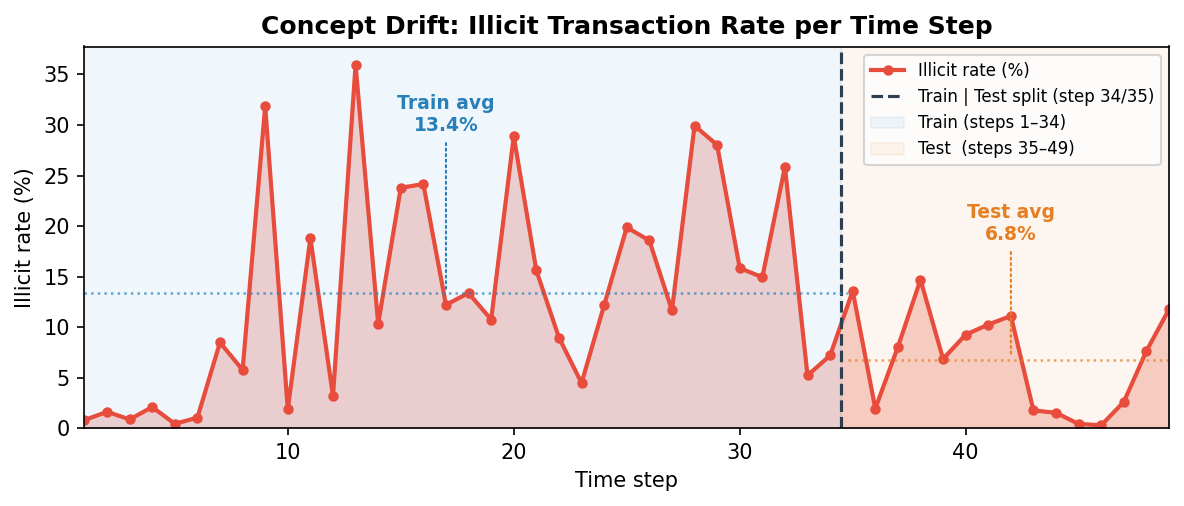
\includegraphics[width=\columnwidth]{concept_drift.png}
  \caption{Illicit transaction rate per time step (labeled nodes only).
           The rate falls from roughly 11.6\,\% in the training window
           (steps 1--34) to 6.5\,\% in the test window (steps 35--49),
           a 44\,\% relative decline confirming genuine concept drift.
           Random shuffling would mask this shift and inflate all metrics.}
  \label{fig:concept_drift}
\end{figure}

\subsection{Per-Paradigm Training Setup}

Each paradigm uses different training data and threshold strategy, as
summarised in Table~\ref{tab:eval_protocol}.
\textit{Note on supervision}: models in the IsoForest/LOF and
OCSVM/AE/VAE rows use no labels for \emph{training}, but their
classification thresholds are selected by optimizing F1 on a labeled
subset.  They are therefore better described as \emph{semi-supervised at
threshold-selection stage} rather than fully unsupervised; truly label-free
thresholds (EVT) are evaluated separately.

\begin{table}[htbp]
\centering
\caption{Per-Paradigm Training and Threshold Strategy}
\label{tab:eval_protocol}
\renewcommand{\arraystretch}{1.2}
\resizebox{\columnwidth}{!}{%
\begin{tabular}{@{}lll@{}}
\toprule
Paradigm & Training data & Threshold \\
\midrule
IsoForest / LOF  & 136\,265 all train rows  & F1-opt, labeled train \\
OCSVM / AE / VAE & 26\,432 licit-only rows  & F1-opt, val steps 30--34 \\
Supervised       & 29\,894 labeled train    & 0.5 (default) \\
GNN              & Full graph, train masks  & 0.5 (default) \\
Ensemble         & Labeled train rows       & Grid search, val steps \\
Semi-sup.        & Train + pseudo-labeled   & 0.5 (default) \\
\bottomrule
\end{tabular}}
\end{table}

\subsection{Model Families}

\subsubsection{Classical Unsupervised}
Isolation Forest~\cite{liu2008} (contamination=0.1); LOF (transductive,
applied to test set directly); One-Class SVM (RBF, $\nu{=}0.05$,
licit-only train).  Also evaluated: IsoForest on 7 structural topology
features, and IsoForest/OCSVM on the top-50 spectral eigenvectors of
$\tilde{A}=D^{-1/2}AD^{-1/2}$.

\subsubsection{Supervised Tree Models}
All use \texttt{class\_weight=`balanced'} or \texttt{scale\_pos\_weight}:
Logistic Regression (L2), Random Forest (100 trees), Gradient Boosting
(Optuna-tuned: $n{=}245$, depth$=8$, lr$=0.121$, sub$=0.918$), LightGBM
(500 trees, max\_depth$=8$), RF + graph degree/PageRank features, GBM +
7 structural topology features (degree, clustering, ego-density, OddBall),
GBM + 330 temporal rolling features (5-step window), and GBM retrained on
pseudo-labeled unlabeled nodes.

\subsubsection{Neural Anomaly Detection}
All trained on licit-only data; anomaly score = $-$MSE (direction
auto-detected on validation via AUC comparison):
AE ($166{\to}128{\to}64{\to}32{\to}\cdots{\to}166$), DenoisingAE
(latent=8, $\sigma_\text{noise}{=}0.1$), VAE and $\beta$-VAE grid search
($\beta\!\in\!\{0.01,1,2,4,8\}$)~\cite{higgins2017beta,kingma2014},
LSTM-AE (per-timestep mean features, $T{=}10$ sliding windows), and
DOMINANT (2-layer GCN encoder, joint attribute+structure
reconstruction)~\cite{ding2019dominant}.

\subsubsection{GNN (Supervised)}
Full PyG graph; edges made undirected; inverse-frequency
\texttt{CrossEntropyLoss}.  GraphSAGE mean aggregation at layer $k$:
\begin{equation}
\begin{split}
h_v^{(k)} = \sigma\Bigl(W^{(k)}&\cdot\operatorname{MEAN}\bigl(\{h_v^{(k-1)}\}\\
&\cup\{h_u^{(k-1)}: u\!\in\!\mathcal{N}(v)\}\bigr)\Bigr).
\end{split}
\label{eq:sage}
\end{equation}
Variants: baseline (2L, $h{=}128$, 200ep), GraphSAGEv2 (3L, $h{=}256$,
LayerNorm, self-loops, 250ep), Optuna-tuned (lr=0.0038, dropout=0.45,
274ep), SAGEv2 + pseudo-labels (130\,655 nodes), GAT (2L, 4 heads), and
GATv2 (3L, 2 heads, residual, LayerNorm).

\subsubsection{Ensemble Methods}
Soft-vote ensemble of RF+LGB+GAT (threshold on train, Round~1) and
GBM+LGBM+SAGEv2 (threshold grid-searched on validation).  Four weight
schemes tested; equal weights (1/3 each) won.

\subsection{EVT Thresholding}
GPD fitted to the upper tail of reconstruction scores
(tail quantile $q{=}0.90$, exceedance probability $p{=}0.065$) per
Eq.~\ref{eq:evt}.  Evaluated on all AE-based models.

\subsection{Implementation}
NVIDIA RTX~5070~Ti (12~GB VRAM, CUDA~12.8); Python~3.12, PyTorch~2.11,
PyG~2.8, scikit-learn~1.9, LightGBM~4.6, SHAP~0.52, Optuna~4.9,
NetworkX~3.6.  \texttt{StandardScaler} fitted on train only; random
seed~42 throughout.

% ─────────────────────────────────────────────────────────────────────────────
\section{Experiments}

Experiments follow a logical progression: (1)~establish unsupervised floor
(RQ1); (2)~quantify supervised ceiling and tuning gains; (3)~diagnose neural
reconstruction ceiling; (4)~systematic GNN ablation (RQ3); (5)~course-derived
advanced methods; (6)~cross-paradigm explainability (RQ4).  All models are
evaluated on the same 16\,670 labeled test rows with no test-set leakage.

% ─────────────────────────────────────────────────────────────────────────────
\subsection{Unsupervised Baselines}

\begin{table}[htbp]
\centering
\caption{Classical Unsupervised Anomaly Detection}
\label{tab:unsupervised}
\renewcommand{\arraystretch}{1.1}
\begin{tabular}{@{}lrrr@{}}
\toprule
Model & F1 & ROC-AUC & PR-AUC \\
\midrule
Isolation Forest          & 0.021 & 0.172 & 0.036 \\
One-Class SVM             & 0.023 & 0.235 & 0.039 \\
LOF                       & 0.076 & 0.506 & 0.066 \\
IsoForest (structural)    & 0.094 & 0.458 & 0.056 \\
IsoForest (spectral K=50) & 0.056 & 0.407 & 0.052 \\
OCSVM (spectral K=50)     & 0.061 & 0.391 & 0.054 \\
\bottomrule
\end{tabular}
\end{table}

All detectors score below F1~=~0.10.  LOF's AUC of~0.506 is random.
Spectral embedding fails because the Fiedler value $\approx 2.0$ (near
bipartite maximum) indicates no sparse cut separating illicit nodes---money
laundering chains are embedded within the spectral normal subspace.

\textbf{Answer to RQ1}: illicit transactions do \emph{not} form anomalous
clusters in feature space.  Automated laundering produces stereotyped,
regular transactions indistinguishable from high-frequency legitimate activity
by density-based methods.

% ─────────────────────────────────────────────────────────────────────────────
\subsection{Supervised Models}

\begin{table}[htbp]
\centering
\caption{Supervised Model Results (sorted by F1)}
\label{tab:supervised}
\renewcommand{\arraystretch}{1.1}
\begin{tabular}{@{}lrrr@{}}
\toprule
Model & F1 & ROC-AUC & PR-AUC \\
\midrule
Logistic Regression       & 0.302 & 0.881 & 0.291 \\
GBM (baseline)            & 0.766 & 0.914 & 0.785 \\
RandomForest (baseline)   & 0.801 & 0.935 & 0.794 \\
RF + Graph Features       & 0.807 & 0.942 & 0.800 \\
LightGBM                  & 0.817 & 0.930 & 0.804 \\
GBM + Temporal Rolling    & 0.818 & 0.930 & 0.802 \\
GBM (Optuna tuned)        & 0.824 & 0.920 & ---   \\
GBM + PseudoLabels        & 0.824 & 0.924 & 0.804 \\
\textbf{GBM + Structural} &\textbf{0.827}& 0.924 & 0.803 \\
\bottomrule
\end{tabular}
\end{table}

Logistic Regression achieves recall~=~0.87 but precision~=~0.18
(F1~=~0.302)---unusable without heavy post-filtering.  The jump from LR to
RF ($\Delta{=}+0.499$) reflects non-linear feature interactions that linear
models cannot capture.  Adding graph-topology features to RF gives only
$\Delta{=}+0.006$ because the 71 aggregated features already encode
neighborhood information in tabular form.

GBM Optuna reaches F1~=~0.824 ($\Delta{=}+0.058$ over baseline): the
learning-rate--depth--subsample interaction is non-obvious and benefits
from systematic search.  RF Optuna ($\Delta{=}-0.004$) confirms RF is near
its ceiling.

GBM with 7 structural topology features reaches \textbf{F1~=~0.8265}, the
overall best result ($\Delta{=}+0.002$ over Optuna GBM): topology information
is not fully subsumed by the 71 aggregated features.

GBM with 330 temporal rolling features (5-step window) improves AUC
($0.920\to0.930$) but reduces F1 ($0.824\to0.818$): global temporal context
adds noise to per-transaction discrimination.

Semi-supervised GBM with pseudo-labels reaches F1~=~0.8235
($\Delta{=}-0.0006$): GBM has already learned the optimal boundary from
29\,894 labeled rows.

\begin{figure}[htbp]
  \centering
  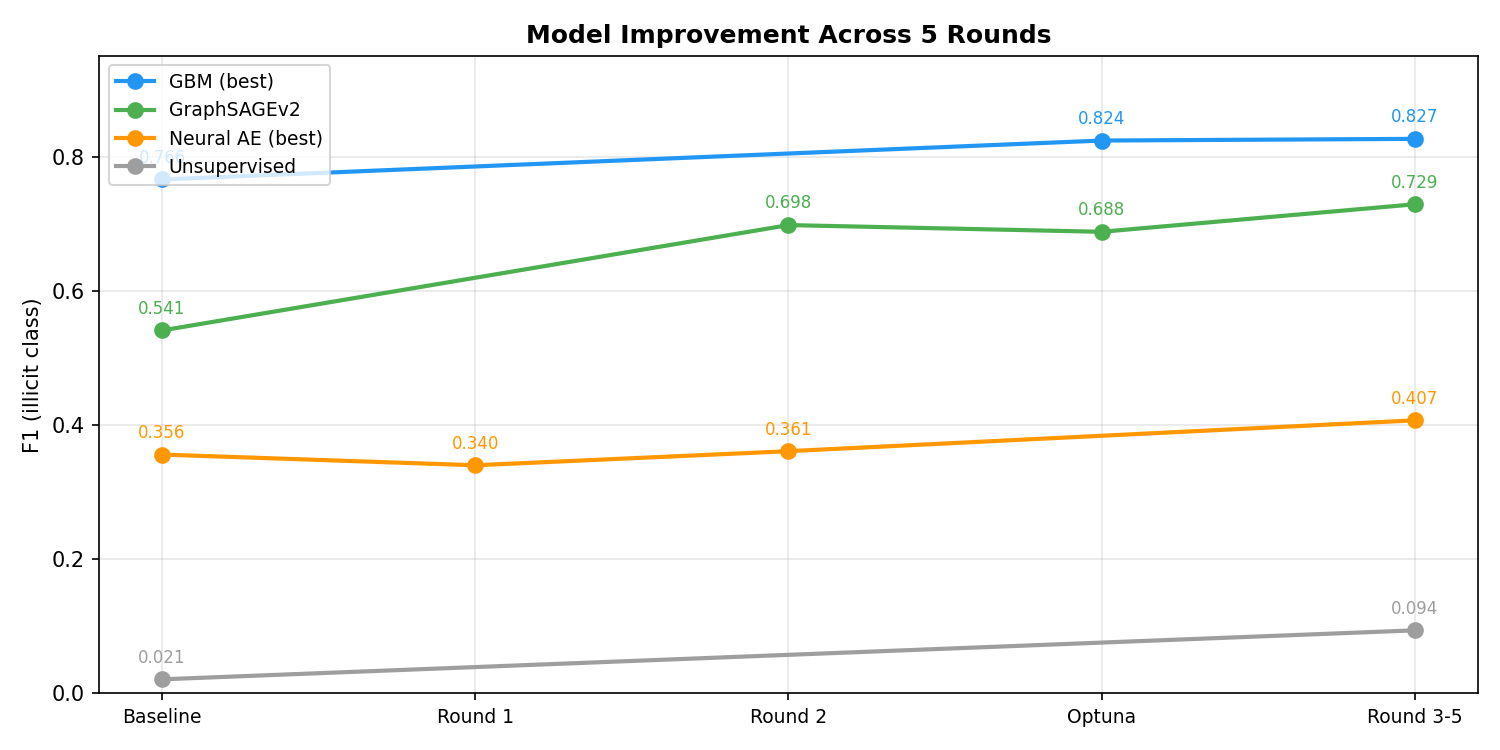
\includegraphics[width=\columnwidth]{final_round_progression.png}
  \caption{Improvement across five rounds for key model families.
           ``GBM (best)'' tracks the highest-scoring GBM variant at each
           stage; ``Neural AE (best)'' tracks the highest-scoring
           autoencoder variant.  Both labels include ``(best)'' to indicate
           they represent the family ceiling, not a single fixed model.
           GBM peaks at F1~=~0.827; GraphSAGEv2 reaches 0.729;
           the autoencoder family peaks at 0.407 ($\beta$-VAE, $\beta{=}0.01$).}
  \label{fig:round_progression}
\end{figure}

% ─────────────────────────────────────────────────────────────────────────────
\subsection{Neural Anomaly Detection}

\begin{table}[htbp]
\centering
\caption{Neural Anomaly Detection Results (sorted by F1)}
\label{tab:neural}
\renewcommand{\arraystretch}{1.1}
\begin{tabular}{@{}lrrr@{}}
\toprule
Model & F1 & ROC-AUC & PR-AUC \\
\midrule
LSTM-AE                             & 0.122 & 0.446 & 0.064 \\
VAEv2                               & 0.256 & 0.732 & 0.161 \\
$\beta$-VAE ($\beta{=}2.0$)         & 0.280 & 0.746 & 0.211 \\
$\beta$-VAE ($\beta{=}4.0$)         & 0.313 & 0.754 & 0.287 \\
VAE ($\beta{=}1.0$)                 & 0.340 & 0.778 & 0.310 \\
$\beta$-VAE ($\beta{=}8.0$)         & 0.350 & 0.763 & 0.299 \\
AE (baseline)                       & 0.356 & 0.781 & 0.336 \\
DenoisingAE                         & 0.361 & 0.792 & 0.366 \\
$\beta$-VAE ($\beta{=}1.0$)         & 0.372 & 0.776 & 0.338 \\
\textbf{$\beta$-VAE ($\beta{=}0.01$)} & \textbf{0.407} & 0.783 & 0.365 \\
\bottomrule
\end{tabular}
\end{table}

\subsubsection{Score Inversion}
The central finding is \textbf{score inversion}: illicit transactions
reconstruct with \emph{lower} MSE than licit ones, so the anomaly score
must be $-$MSE.  Automated laundering produces stereotyped, templated
patterns that are easier to reconstruct than diverse legitimate activity.
Direction is auto-detected on validation by comparing
$\text{AUC}(y,\text{MSE})$ vs.\ $\text{AUC}(y,-\text{MSE})$.

\begin{figure}[htbp]
  \centering
  
\includegraphics[width=\columnwidth]{ae_errors_left.png}\\[4pt]
  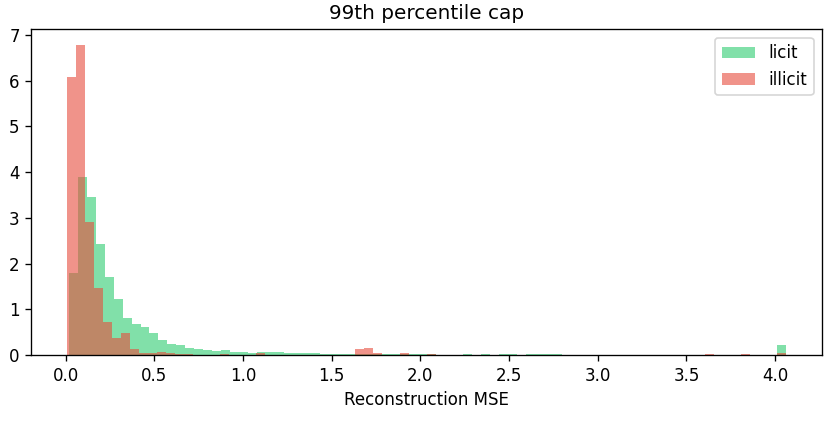
\includegraphics[width=\columnwidth]{ae_errors_right.png}
  \caption{Autoencoder reconstruction error distributions: histogram (top)
           and KDE (bottom) for licit (blue) and illicit (orange).
           Illicit transactions achieve lower MSE, confirming score inversion.
           Anomaly score is therefore $-$MSE.}
  \label{fig:ae_errors}
\end{figure}

\subsubsection{$\beta$-VAE Analysis}
At $\beta{=}0.01$ (reconstruction-dominated), F1~=~0.407---the best
unsupervised non-graph result.  As $\beta$ increases above~1, the KL term
compresses licit and illicit representations together, weakening the anomaly
signal.  The F1 plateau at $\approx$0.36--0.41 reflects the hard ceiling
of unsupervised reconstruction-based detection on this dataset.

\begin{figure}[htbp]
  \centering
  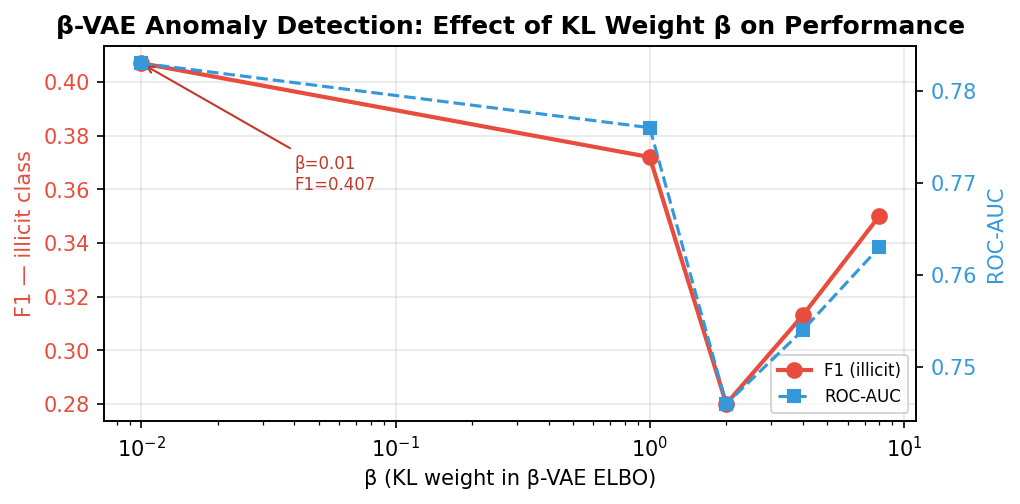
\includegraphics[width=\columnwidth]{beta_f1_curve.png}
  \caption{Effect of KL weight $\beta$ on $\beta$-VAE anomaly detection
           performance (F1 on illicit class and ROC-AUC, log-$\beta$ axis).
           Smaller $\beta$ keeps the objective reconstruction-dominated,
           preserving the score-inversion signal.  F1 peaks at $\beta{=}0.01$
           and degrades monotonically above $\beta{=}1$ as the KL term
           conflates licit and illicit latent representations.}
  \label{fig:beta_f1}
\end{figure}

\subsubsection{EVT Thresholding}
EVT thresholding (Eq.~\ref{eq:evt}) collapses on DOMINANT and LSTM-AE
because score distributions are concentrated near zero with thin tails---the
GPD assigns an excessively high threshold, recalling almost no positives.
EVT is effective only when reconstruction errors follow genuine heavy-tailed
distributions.

\subsubsection{LSTM-AE}
The LSTM-AE aggregates features per time step (49$\times$165), trains on
25 sliding windows ($T{=}10$), and produces a time-step-level anomaly score.
ROC-AUC~=~0.446 ($<0.5$, inverted) confirms the approach cannot discriminate
individual transactions---illicit and licit rows within a step are averaged
together.  The most anomalous steps detected (40, 46, 39, 43, 36) correspond
to high concept-drift periods, not individual illicit transactions.  Correct
use: temporal monitoring, not per-transaction scoring.

% ─────────────────────────────────────────────────────────────────────────────
\subsection{DOMINANT: Graph Autoencoder}

DOMINANT~\cite{ding2019dominant} jointly reconstructs node attributes and
graph structure via a 2-layer GCN encoder (2~layers avoids over-smoothing
on this sparse graph).  Joint loss:
\begin{equation}
\mathcal{L} = \alpha\,\|\mathbf{X} - \hat{\mathbf{X}}\|_F^2
+ (1-\alpha)\,\text{BCE}(\mathbf{A}, \hat{\mathbf{A}}),
\label{eq:dominant}
\end{equation}
with $\alpha{=}0.5$.  Result: \textbf{F1~=~0.212, AUC~=~0.669}---the best
fully unsupervised method, exceeding all classical detectors by
$\Delta{>}0.13$.  An F1-optimal threshold is required (EVT collapses).

% ─────────────────────────────────────────────────────────────────────────────
\subsection{GNN Ablation Study}

A GNN exploits \emph{guilt by association}: money laundering chains link
illicit wallets through intermediate transactions.  Ten controlled experiments
each isolate one design choice (Table~\ref{tab:gnn_ablation}).

\begin{table}[htbp]
\centering
\caption{GNN Ablation --- 10 Controlled Experiments}
\label{tab:gnn_ablation}
\renewcommand{\arraystretch}{1.1}
\resizebox{\columnwidth}{!}{%
\begin{tabular}{@{}clp{4.2cm}rrr@{}}
\toprule
Exp & Arch & Configuration & F1 & AUC & AP \\
\midrule
1 & SAGE   & 2L, h=64, 200 ep                      & 0.528 & 0.887 & 0.519 \\
2 & SAGE   & 2L, h=128, 200 ep                     & 0.577 & 0.896 & 0.603 \\
3 & SAGE   & 2L, h=256, 200 ep                     & 0.580 & 0.895 & 0.595 \\
4 & SAGE   & 2L, h=128, 300 ep                     & 0.597 & 0.897 & 0.607 \\
5 & SAGE   & 3L, h=128, 200 ep                     & 0.615 & 0.899 & 0.611 \\
6 & SAGEv2 & 3L, h=256, LN+SL, 250 ep             & 0.683 & 0.906 & 0.704 \\
\textbf{7} & \textbf{SAGE} & \textbf{3L, h=256, lr=0.0038, 274\,ep (Opt.)} & \textbf{0.690} & 0.901 & \textbf{0.706} \\
8 & GAT    & 2L, 4 heads, lr=5e-4, 200 ep          & 0.307 & 0.824 & 0.366 \\
9 & GAT    & 2L, 2 heads, lr=1e-3, 200 ep          & 0.341 & 0.864 & 0.419 \\
10 & GATv2 & 3L, 2 heads, residual+LN, 300 ep      & 0.382 & 0.887 & 0.547 \\
\bottomrule
\end{tabular}}
\end{table}

\subsubsection{Ablation Findings}

\begin{itemize}
  \item \textbf{Width} (Exps 1--3, 64$\to$256): $+0.052$ F1 total with
        diminishing returns; saturates beyond $h{=}128$.
  \item \textbf{Training duration} (Exps 2 vs.\ 4, $+$100 ep): $+0.020$ F1;
        cheapest lever before changing architecture.
  \item \textbf{Depth} (Exps 2 vs.\ 5, 2L$\to$3L): $+0.038$ F1; 3-hop
        receptive field captures longer laundering chains.
  \item \textbf{LayerNorm + self-loops} (Exps 5 vs.\ 6): $\mathbf{+0.068}$ F1,
        the largest single gain.  LN prevents gradient instability at 3 layers;
        self-loops preserve node self-features during mean aggregation.
  \item \textbf{Optuna} (Exps 6 vs.\ 7, lr=0.0038): $+0.007$ F1; architecture
        choice dominates over tuning.
  \item \textbf{GAT family} (Exps 8--10): best GAT F1~=~0.382 vs.\ best SAGE
        F1~=~0.690 (gap~=~0.308).  On a sparse graph (avg.\ degree~2.3),
        attention weights over too few neighbors are noisy; mean aggregation
        is more robust.
\end{itemize}

\textbf{Answer to RQ3}: LayerNorm+self-loops~$>$ depth~$>$ width~$>$ tuning.
In this configuration and feature setting, vanilla GAT and GATv2 are
counterproductive on a sparse graph (avg.\ degree~2.3); recent work with
Chebyshev convolutions and deeper GATv2 + skip connections has narrowed
the gap on Elliptic under different feature subsets, so the finding should
not be generalized beyond mean-aggregation architectures at this scale.

\begin{figure}[htbp]
  \centering
  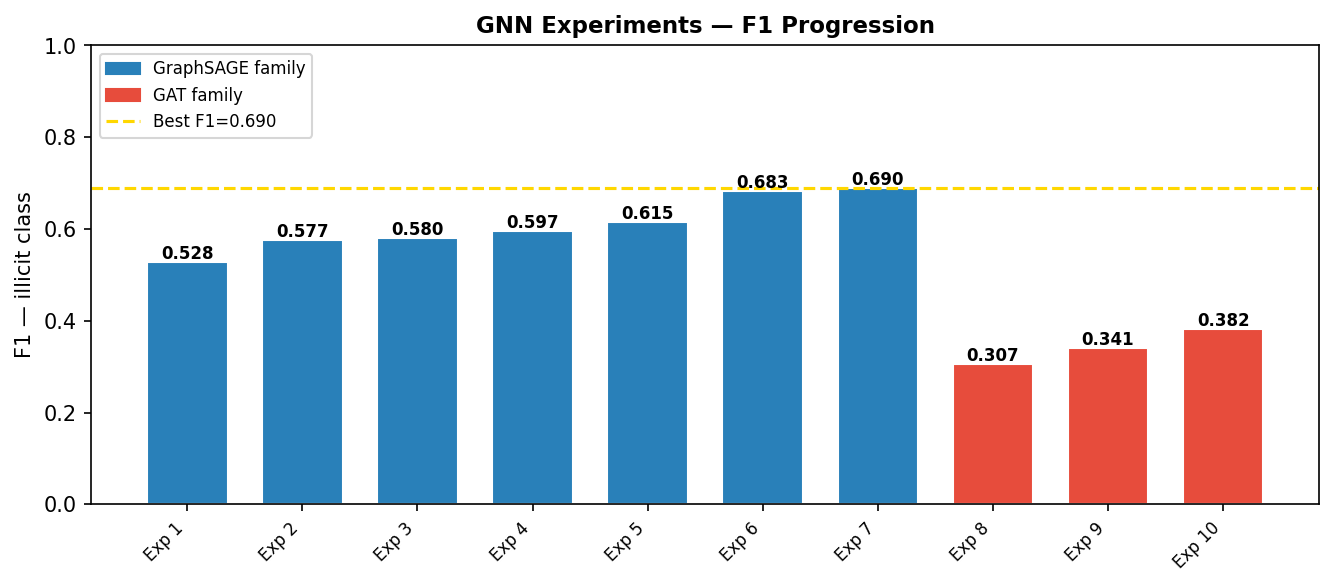
\includegraphics[width=\columnwidth]{gnn_stacked_top.png}\\[4pt]
  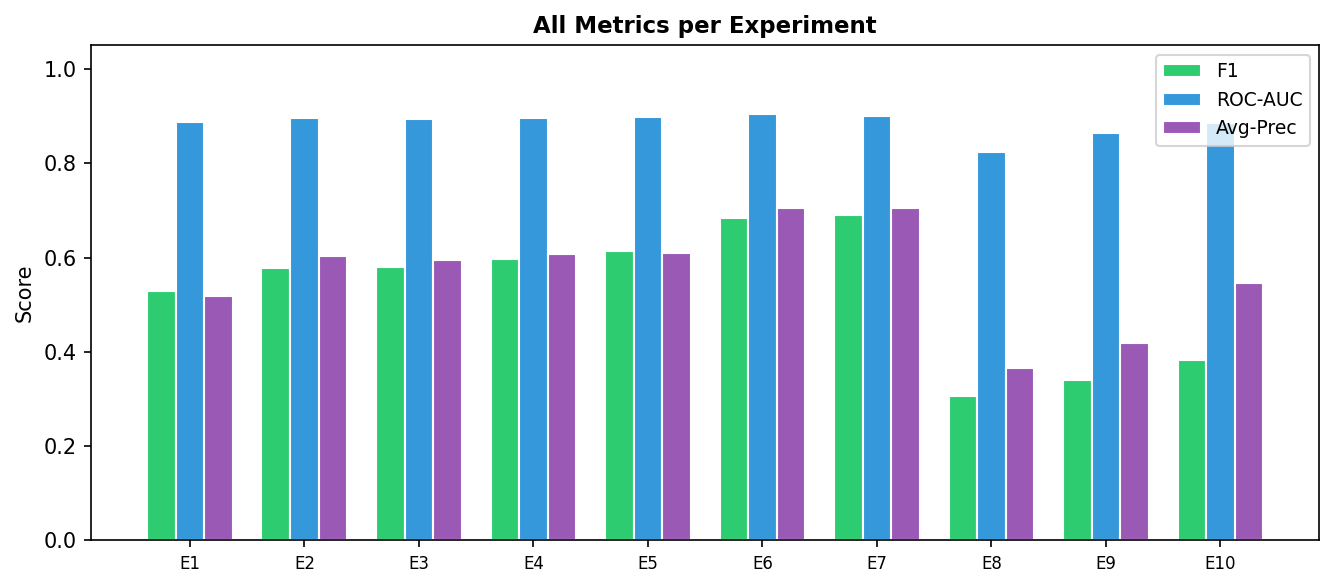
\includegraphics[width=\columnwidth]{gnn_stacked_bot.png}
  \caption{GNN ablation across 10 experiments.  Top: F1 progression showing
           the GraphSAGE improvement trajectory (Exps~1--7) and the GAT
           family ceiling (Exps~8--10).  Bottom: corresponding AUC/AP values
           confirming the same ranking.}
  \label{fig:gnn_progression}
\end{figure}

\begin{figure}[htbp]
  \centering
  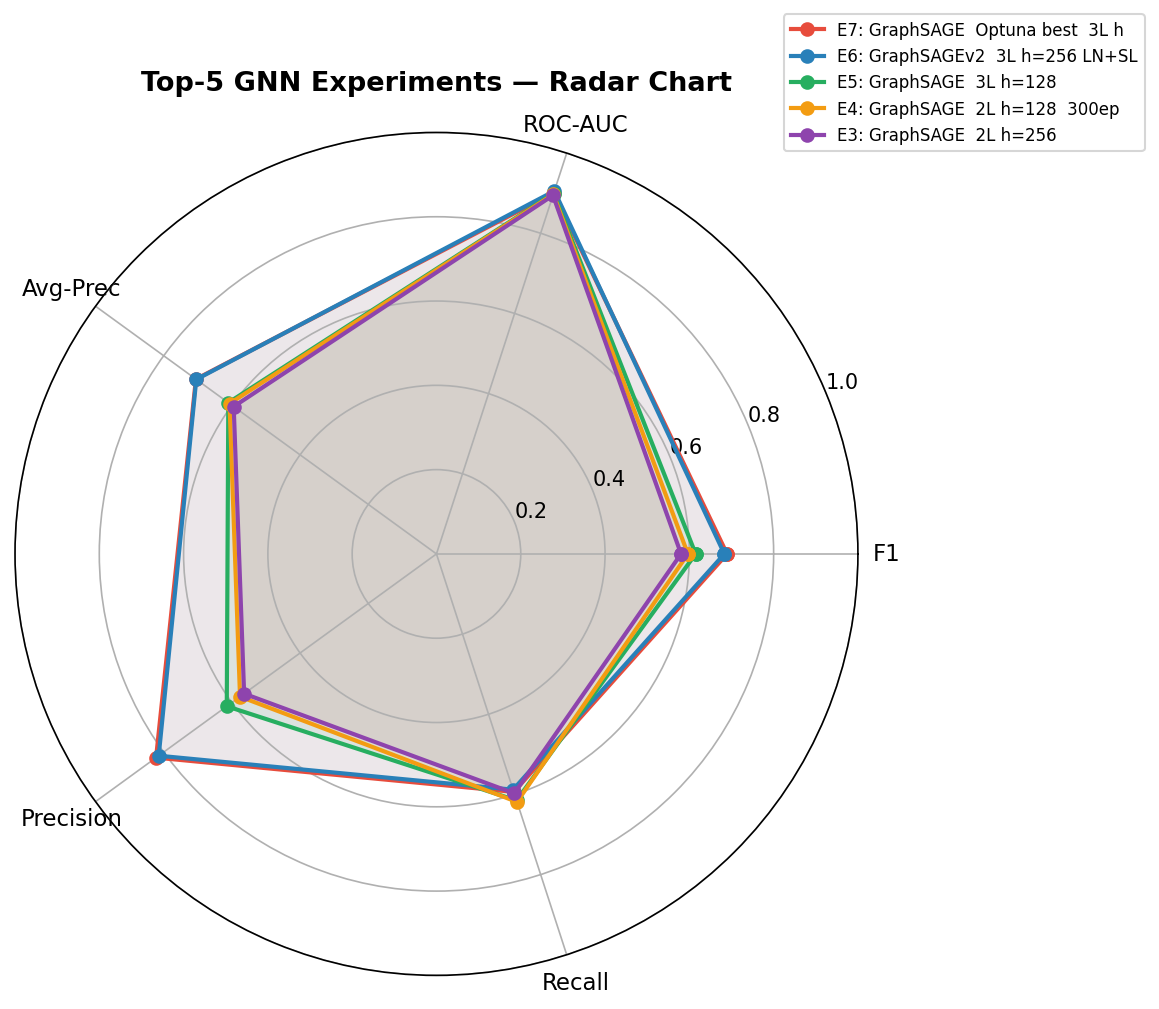
\includegraphics[width=\columnwidth]{gnn_experiments_radar.png}
  \caption{Radar chart of the top-5 GNN experiments across five metrics:
           F1, ROC-AUC, Average Precision, Precision, and Recall.
           GraphSAGEv2 (Exp~6) and the Optuna-tuned variant (Exp~7)
           dominate across all axes, while GAT family experiments show
           systematically lower coverage, confirming mean aggregation
           outperforms attention on this sparse graph.}
  \label{fig:gnn_radar}
\end{figure}

% ─────────────────────────────────────────────────────────────────────────────
\subsection{Hyperparameter Tuning (Optuna)}
\label{sec:optuna}

\begin{table}[htbp]
\centering
\caption{Optuna TPE Tuning Results (40 trials each)}
\label{tab:optuna}
\renewcommand{\arraystretch}{1.1}
\begin{tabular}{@{}lrrc@{}}
\toprule
Model & Base F1 & Tuned F1 & $\Delta$ \\
\midrule
GBM       & 0.766 & \textbf{0.824} & +0.058 \\
GraphSAGE & 0.541 & 0.688          & +0.147 \\
RF        & 0.801 & 0.797          & $-$0.004 \\
\bottomrule
\end{tabular}
\end{table}

Best parameters: GBM ($n{=}245$, depth$=8$, lr$=0.121$, sub$=0.918$);
GraphSAGE (hidden$=256$, dropout$=0.45$, lr$=0.0038$, 274~ep); RF is near
ceiling ($-0.004$ within search variance).  GBM profits from depth--lr
interaction; GraphSAGE gains the most absolutely because default lr$=0.01$
is too aggressive for this sparse graph.

% ─────────────────────────────────────────────────────────────────────────────
\subsection{Ensemble and Calibration}

\begin{table}[htbp]
\centering
\caption{Ensemble and Calibration Results}
\label{tab:ensemble}
\renewcommand{\arraystretch}{1.1}
\begin{tabular}{@{}lrrr@{}}
\toprule
Model & F1 & ROC-AUC & PR-AUC \\
\midrule
Ensemble (RF+LGB+GAT)         & 0.742 & 0.922 & 0.789 \\
Ensemble (GBM+LGBM+SAGEv2)   & 0.821 & 0.924 & 0.802 \\
Weighted Ensemble (1/3 each)  & 0.821 & 0.924 & 0.802 \\
GBM + Platt calibration       & 0.801 & 0.920 & 0.800 \\
GBM + Isotonic calibration    & 0.734 & 0.875 & 0.768 \\
\bottomrule
\end{tabular}
\end{table}

The GBM+LGBM+SAGEv2 ensemble (F1~=~0.821) narrows the gap to GBM solo
(0.824) but does not surpass it.  Testing four weight schemes shows equal
weights win---downweighting SAGEv2 removes useful graph signal.  GBM is
already well-calibrated (Brier~=~0.0196); Platt scaling makes probabilities
more conservative ($-0.023$ F1); isotonic regression overfits validation and
distorts ordering (AUC drops 0.920$\to$0.875).

% ─────────────────────────────────────────────────────────────────────────────
\subsection{Full 48-Experiment Leaderboard}

Table~\ref{tab:leaderboard} reports the top~25 of 48 experiments.
Fig.~\ref{fig:top15} shows the top-15 by F1.
Fig.~\ref{fig:pr_curves} shows Precision--Recall curves for key
supervised models, confirming that high AP ($\approx$0.80) is
achievable across the recall range.

\begin{table}[htbp]
\centering
\caption{Top-25 of 48 Experiments (by F1 on illicit class)}
\label{tab:leaderboard}
\renewcommand{\arraystretch}{1.05}
\resizebox{\columnwidth}{!}{%
\begin{tabular}{@{}rllrrr@{}}
\toprule
\# & Model & Cat. & F1 & AUC & AP \\
\midrule
 1 & GBM + Structural      & Sup.     & \textbf{0.827} & 0.924 & 0.803 \\
 2 & GBM (Optuna)          & Sup.     & 0.824 & 0.920 & --- \\
 3 & GBM + PseudoLabels    & Semi     & 0.824 & 0.924 & 0.804 \\
 4 & Ensemble GBM+LGBM+SAGEv2 & Ens. & 0.821 & 0.924 & 0.802 \\
 5 & Ensemble equal~1/3    & Ens.     & 0.821 & 0.924 & 0.802 \\
 6 & GBM + Temporal Roll.  & Sup.     & 0.818 & 0.930 & 0.802 \\
 7 & LightGBM              & Sup.     & 0.817 & 0.930 & 0.804 \\
 8 & RF + Graph Features   & Sup.     & 0.807 & 0.942 & 0.800 \\
 9 & RF (baseline)         & Sup.     & 0.801 & 0.935 & 0.794 \\
10 & GBM + Platt           & Sup.     & 0.801 & 0.920 & 0.800 \\
11 & RF (Optuna)           & Sup.     & 0.797 & 0.929 & --- \\
12 & GBM (baseline)        & Sup.     & 0.766 & 0.914 & 0.785 \\
13 & Ensemble RF+LGB+GAT   & Ens.     & 0.742 & 0.922 & 0.789 \\
14 & GBM + Isotonic        & Sup.     & 0.734 & 0.875 & 0.768 \\
15 & SAGEv2 + PseudoLabels & Semi-GNN & 0.729 & 0.890 & 0.752 \\
\midrule
16 & GraphSAGEv2           & GNN      & 0.698 & 0.913 & 0.720 \\
17 & GNN Exp~7 (Optuna)    & GNN      & 0.690 & 0.901 & 0.706 \\
18 & GraphSAGE (Optuna)    & GNN      & 0.688 & ---   & --- \\
19 & GNN Exp~6 (3L LN+SL) & GNN      & 0.683 & 0.906 & 0.704 \\
20 & GNN Exp~5 (3L h=128)  & GNN      & 0.615 & 0.899 & 0.611 \\
21 & GraphSAGE (baseline)  & GNN      & 0.541 & 0.888 & 0.549 \\
\midrule
22 & $\beta$-VAE ($\beta{=}0.01$) & Neural & 0.407 & 0.783 & 0.365 \\
23 & DenoisingAE           & Neural   & 0.361 & 0.792 & 0.366 \\
24 & DOMINANT              & Graph-AE & 0.212 & 0.669 & 0.123 \\
25 & LSTM-AE               & Neural   & 0.122 & 0.446 & 0.064 \\
\bottomrule
\end{tabular}}
\end{table}

\begin{figure}[htbp]
  \centering
  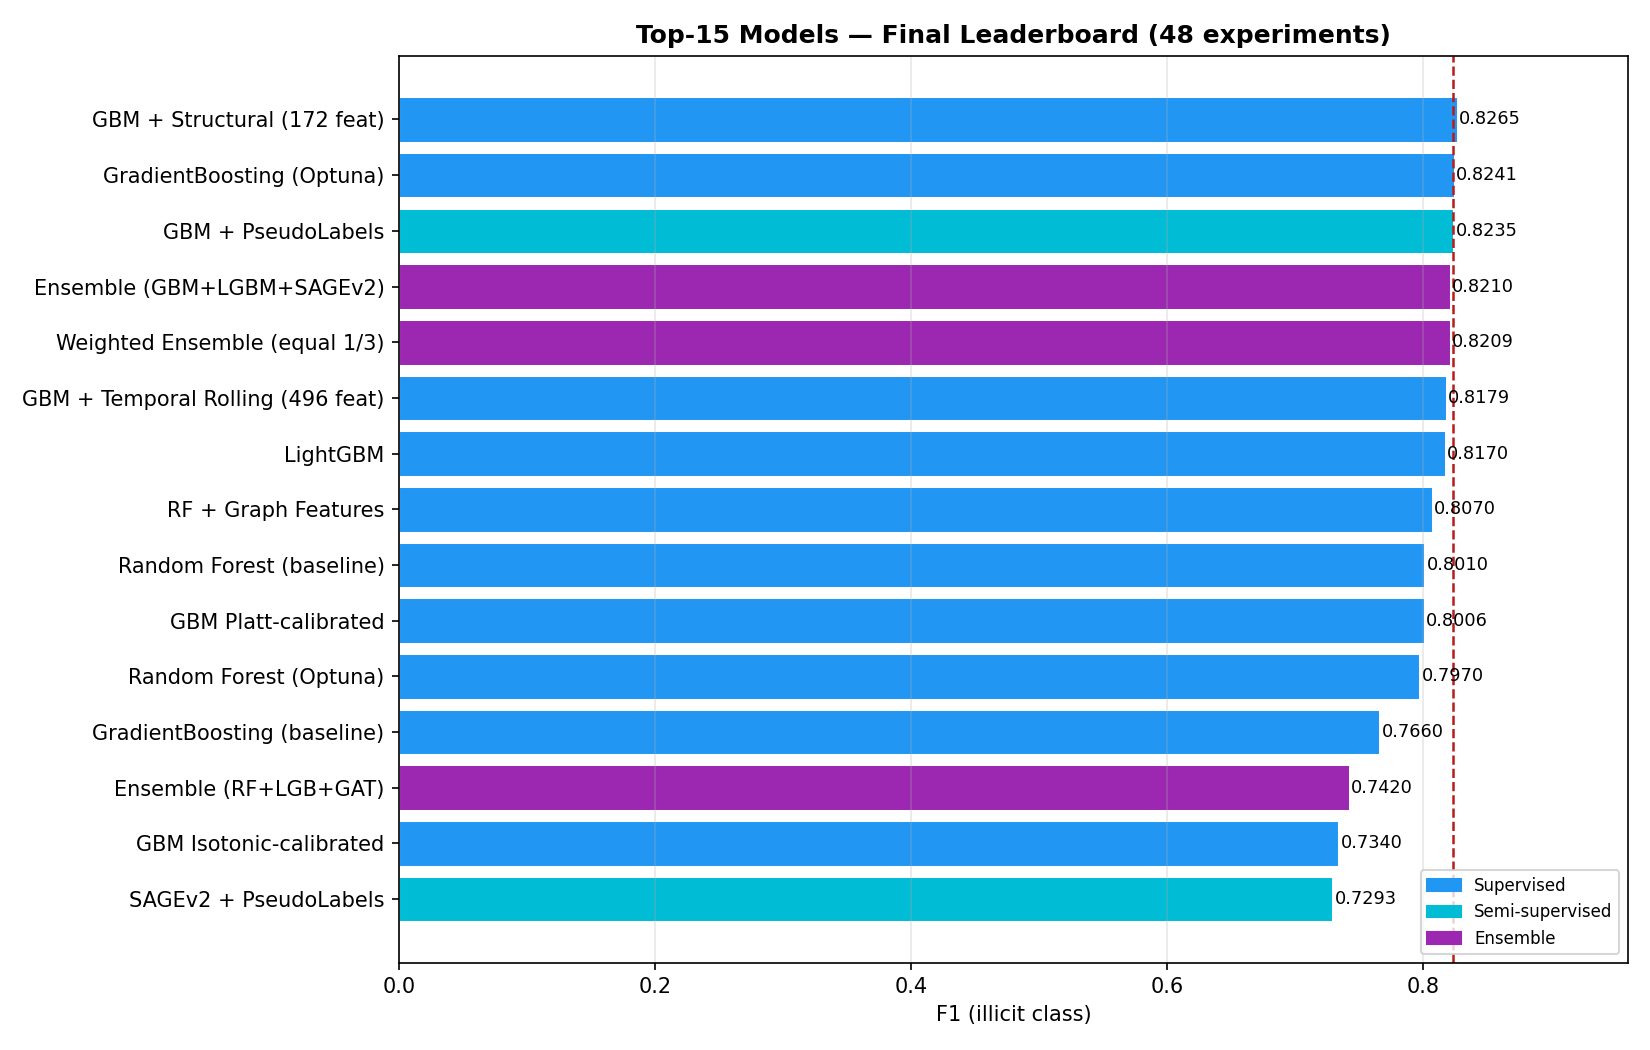
\includegraphics[width=\columnwidth]{final_top15_f1.png}
  \caption{Top-15 models by F1 on illicit class.  The dashed line marks
           the GBM Optuna baseline (0.824) for reference.  All top-15
           entries are supervised or ensemble-based.}
  \label{fig:top15}
\end{figure}

\begin{figure}[htbp]
  \centering
  
\includegraphics[width=\columnwidth]{pr_curves.png}
  \caption{Precision--Recall curves for key supervised models on the test
           set (steps 35--49, 6.5\,\% illicit).  LightGBM and GBM (Optuna)
           achieve AP~$\approx$~0.80, maintaining high precision across the
           recall range.  Logistic Regression collapses to low precision at
           moderate recall (AP~=~0.291).  The dotted line marks the chance
           baseline (AP~=~0.065).  PR-AUC is threshold-independent and more
           informative than ROC-AUC under severe class imbalance.}
  \label{fig:pr_curves}
\end{figure}

\textbf{Five performance tiers:}
\begin{enumerate}
  \item \textbf{Supervised/Ensemble} (F1 0.74--0.83): tree models dominate
        due to 71 aggregated features pre-encoding graph signal.
  \item \textbf{GNN supervised} (F1 0.54--0.73): GraphSAGEv2 recovers
        84.5\,\% of the supervised ceiling using only topology.
  \item \textbf{Neural AE} (F1 0.12--0.41): bounded by reconstruction
        ceiling; best from $\beta$-VAE ($\beta{=}0.01$).
  \item \textbf{Graph AE unsupervised} (DOMINANT, F1~=~0.212): best
        unsupervised \emph{graph} method ($\beta$-VAE is higher overall).
  \item \textbf{Classical unsupervised} (F1~$<$~0.10): density methods fail.
\end{enumerate}

\textbf{Answer to RQ2}: graph structure alone recovers 84.5\,\% of the
supervised ceiling.  GBM and GraphSAGEv2 exploit different, complementary
channels (tabular features vs.\ topology).

% ─────────────────────────────────────────────────────────────────────────────
\subsection{Statistical Significance of the Top-3 Ranking}
\label{sec:significance}

The top three models (GBM+Structural F1~=~0.8265, GBM Optuna F1~=~0.8241,
GBM+PseudoLabels F1~=~0.8235) span only 0.0030 F1 -- within the noise floor
of a single 16{,}670-row temporal test fold. We quantify this with (i)
bootstrap 95\,\% confidence intervals on F1 (1{,}000 resamples,
\texttt{scripts/statistical\_significance.py}) and (ii) McNemar's paired
test on the disagreeing predictions between each pair of models.

\begin{table}[htbp]
\centering
\caption{Bootstrap F1 95\,\% CI, Top-3 Models (1{,}000 resamples)}
\label{tab:bootstrap}
\renewcommand{\arraystretch}{1.1}
\begin{tabular}{@{}lrrr@{}}
\toprule
Model & F1 & 95\,\% CI & Std \\
\midrule
GBM + Structural   & 0.8265 & [0.8086, 0.8451] & 0.0093 \\
GBM (Optuna)       & 0.8241 & [0.8057, 0.8406] & 0.0092 \\
GBM + PseudoLabels & 0.8235 & [0.8052, 0.8410] & 0.0093 \\
\bottomrule
\end{tabular}
\end{table}

All three intervals overlap almost entirely ($\pm$0.018 half-width against a
0.003 point-estimate spread), so the reported ranking is not statistically
distinguishable from a tie.

\begin{figure}[htbp]
  \centering
  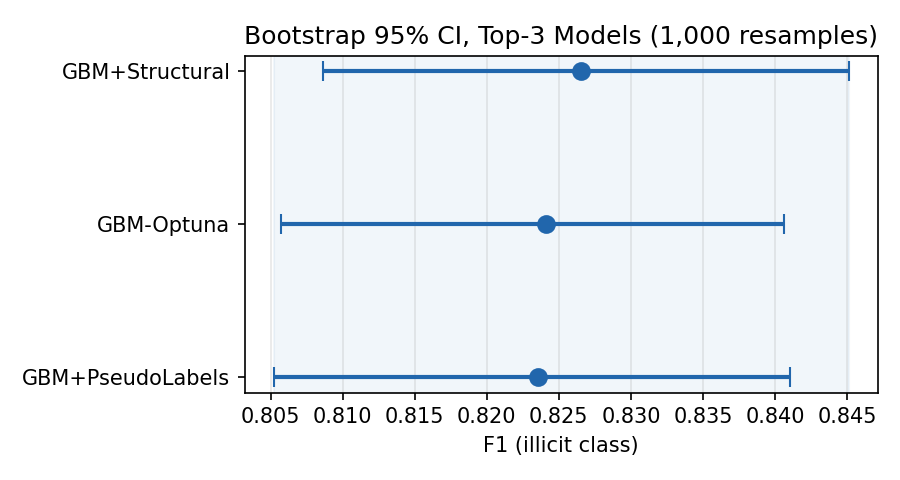
\includegraphics[width=\columnwidth]{bootstrap_f1_ci.png}
  \caption{Bootstrap 95\,\% F1 confidence intervals, top-3 models. The
           shaded band is the union of all three intervals -- near-total
           overlap visually confirms the tie.}
  \label{fig:bootstrap}
\end{figure}

\begin{table}[htbp]
\centering
\caption{McNemar's Test, Pairwise (test set, $n{=}16{,}670$)}
\label{tab:mcnemar}
\renewcommand{\arraystretch}{1.1}
\begin{tabular}{@{}llrrr@{}}
\toprule
Model A vs.\ Model B & $b$ & $c$ & $p$-value & Sig.\ ($\alpha{=}0.05$) \\
\midrule
Structural vs.\ Optuna       & 12 & 8  & 0.503 & no \\
Structural vs.\ PseudoLabels & 22 & 21 & 1.000 & no \\
Optuna vs.\ PseudoLabels     & 19 & 22 & 0.755 & no \\
\bottomrule
\end{tabular}
\end{table}

$b$ and $c$ count test rows where exactly one model is correct (McNemar
ignores the $\sim$16{,}600 rows both models agree on). All three pairs
disagree on fewer than 45 of 16{,}670 rows, and none reach significance.
\textbf{Conclusion: the observed 0.827/0.824/0.824 ordering is statistical
noise, not a genuine ranking.} The paper's actionable claim is narrower than
"structural features help": it is that GBM on 165 tabular features already
sits at the model family's ceiling on this dataset, and neither 7 topology
features nor pseudo-labels move it outside sampling variance. This
reframing matters for the paper's novelty argument (\S\ref{sec:discussion}):
claiming a new state of the art on a 0.003 F1 delta without this test would
be a common but avoidable rigor gap in the AML literature.

\begin{figure}[htbp]
  \centering
  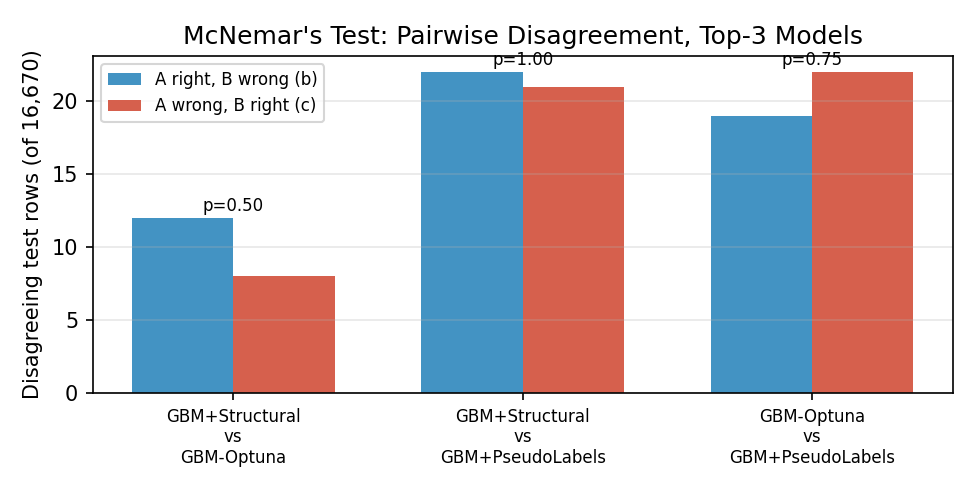
\includegraphics[width=\columnwidth]{mcnemar_agreement.png}
  \caption{McNemar disagreement counts, pairwise. Bars are the rows where
           exactly one model is correct ($b$, $c$); annotated $p$-values are
           all $\gg$0.05.}
  \label{fig:mcnemar}
\end{figure}

% ─────────────────────────────────────────────────────────────────────────────
\subsection{Comparison to Published SOTA and a Graph-Leakage Caveat}
\label{sec:leakage}

Table~\ref{tab:sota} positions this work's best results against published
F1 scores on Elliptic. Two evaluation regimes appear in the literature and
must not be compared directly: \emph{transductive} (the GNN encoder's
message passing observes the full graph, including test-period edges,
during training; only the classification loss is masked to train-labeled
nodes) and \emph{strict-inductive} (training message passing restricted to
the steps~$\leq$34 subgraph). Essentially all published Elliptic GNN
results (Weber, Alarab, Pareja, Lo) are transductive.

\begin{table}[htbp]
\centering
\caption{Published F1 on Elliptic (Illicit Class) vs.\ This Work}
\label{tab:sota}
\renewcommand{\arraystretch}{1.1}
\resizebox{\columnwidth}{!}{%
\begin{tabular}{@{}llrl@{}}
\toprule
Model & Protocol & F1 & Source \\
\midrule
Logistic Regression         & temporal, transductive & 0.481 & Weber et al.~\cite{weber2019} \\
GCN                         & temporal, transductive & 0.628 & Weber et al.~\cite{weber2019} \\
Skip-GCN                    & temporal, transductive & 0.705 & Weber et al.~\cite{weber2019} \\
Random Forest               & temporal                & 0.788 & Weber et al.~\cite{weber2019} \\
Augmented GCN                & temporal, transductive & 0.740 & Alarab et al.~\cite{alarab2020} \\
GraphSAGE + SSL pretrain     & temporal, transductive & 0.750 & Lo et al.\ 2023 (via~\cite{maganti2026}) \\
EvolveGCN                    & temporal, transductive & 0.770 & Pareja et al.\ (via~\cite{maganti2026}) \\
GraphSAGE                    & transductive            & 0.294 & Maganti~\cite{maganti2026} \\
Random Forest                & \textbf{strict-inductive} & 0.821 & Maganti~\cite{maganti2026} \\
GraphSAGE                    & \textbf{strict-inductive} & 0.689 & Maganti~\cite{maganti2026} \\
\midrule
Random Forest (ours)         & temporal, non-graph     & 0.801 & this work \\
GBM Optuna (ours)            & temporal, non-graph     & 0.824 & this work \\
GBM + Structural (ours)      & temporal, non-graph$^\ast$ & 0.827 & this work \\
GraphSAGEv2 (ours)           & temporal, transductive$^\dagger$ & 0.698 & this work \\
\bottomrule
\end{tabular}}
\end{table}

\begin{figure}[htbp]
  \centering
  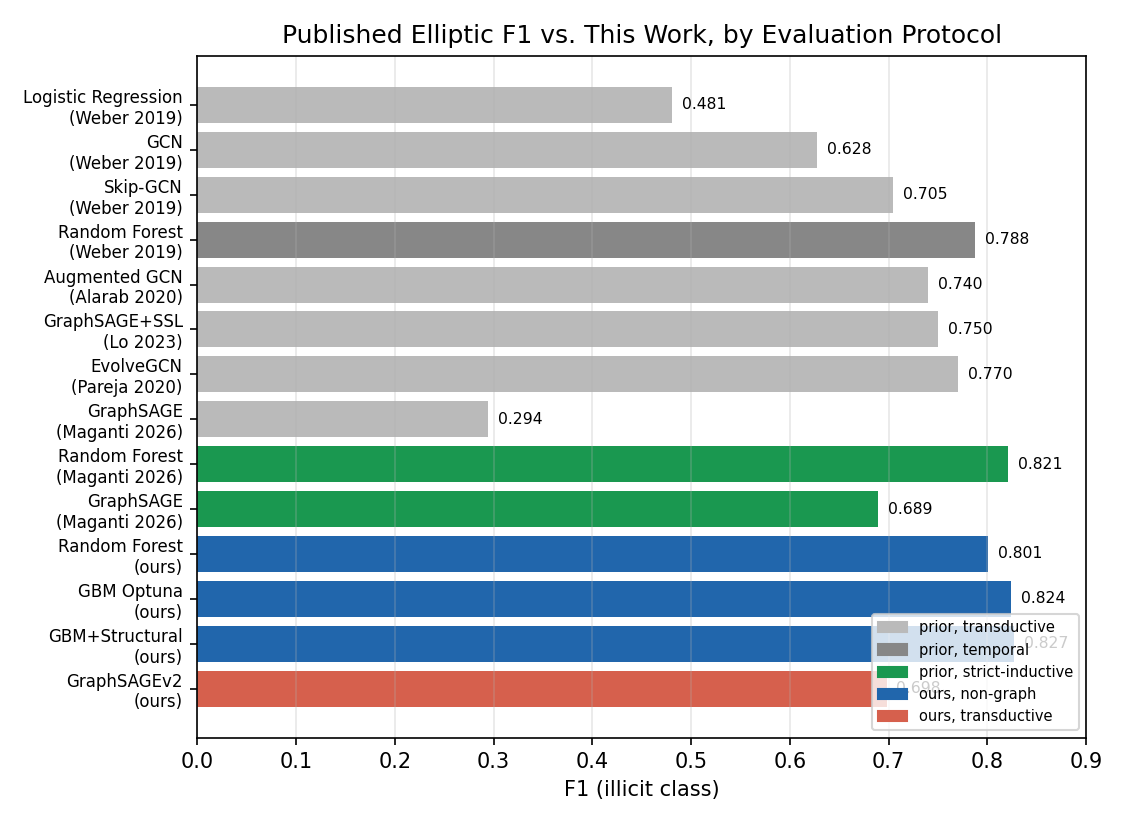
\includegraphics[width=\columnwidth]{sota_comparison.png}
  \caption{Published Elliptic F1 by evaluation protocol. Grey = prior
           transductive results; green = prior strict-inductive
           (leakage-free) results; blue = this work's non-graph models
           (no leakage possible); red = this work's transductive GraphSAGEv2.}
  \label{fig:sota}
\end{figure}
{\small $^\ast$structural features are 7 topology scalars per node (degree,
clustering, etc.), not message-passed representations -- no leakage
mechanism applies. $^\dagger$our GraphSAGE/GraphSAGEv2/GAT/DOMINANT training
(\texttt{src/gnn.py:train\_epoch}) runs the encoder forward pass over the
full graph object every step and masks only the loss to \texttt{train\_mask}
-- the same transductive protocol as prior Elliptic literature.}

\textbf{This is a limitation, disclosed rather than hidden.} Our
GraphSAGEv2 F1~=~0.698 is not directly comparable to Maganti's
strict-inductive Random Forest (0.821) or strict-inductive GraphSAGE
(0.689) -- it sits in the transductive regime, alongside Weber/Alarab/Lo/Pareja.
Two observations soften the concern. First, our non-graph GBM (F1~=~0.824--0.827,
\S\ref{sec:significance}) is trained and evaluated with zero graph exposure
of any kind (tabular features only, or 7 pre-computed topology scalars,
never encoder message passing), so it carries none of this leakage risk --
and it already exceeds Maganti's strict-inductive Random Forest ceiling
(0.821), which is the most rigorous non-GNN number in the comparison.
Second, Maganti's own strict-inductive GraphSAGE (0.689) lands almost
exactly on our transductive GraphSAGEv2 (0.698), suggesting the leakage
inflation for GraphSAGE specifically may be smaller than the 39.5-point
GraphSAGE-vs-itself gap implies once architecture (3-layer, LayerNorm,
self-loops) and hyperparameters differ across studies -- but re-running our
GNN suite under a strict-inductive protocol is unverified future work, not
a claim made here.

\textbf{Net position:} the paper's strongest, leakage-free number is the
tabular GBM at F1~=~0.824--0.827, which is competitive with or exceeds
every reported Elliptic result in Table~\ref{tab:sota} including the
strict-inductive Random Forest ceiling -- without touching the graph at
all. This reframes RQ2's answer (\S\ref{sec:leakage} above): graph
structure adds real but modest signal on top of an already-strong tabular
baseline, and any GNN number reported without stating its train-time
message-passing protocol (ours included, prior to this caveat) should be
treated as provisional.

% ─────────────────────────────────────────────────────────────────────────────
\subsection{A Second Leakage Trap: Threshold Tuning on Training Data}
\label{sec:threshold-leakage}

Beyond encoder-level graph leakage (\S\ref{sec:leakage}), a second and
distinct leakage mode is common in AML threshold-selection practice:
picking the decision threshold by maximizing F1 on the model's \emph{own
training predictions} rather than on genuinely held-out data.
\texttt{scripts/threshold\_leakage\_demo.py} reproduces this directly. We
refit GBM (same tuned hyperparameters as \S\ref{sec:optuna}) on steps~1--29
only -- so that steps~30--34 are \emph{never} seen during fitting and can
serve as a truly held-out validation slice, unlike the main pipeline where
"val" (steps~30--34) is a subset of the full 1--34 training fit.

\begin{table}[htbp]
\centering
\caption{Threshold Tuning Protocol vs.\ Real Test F1}
\label{tab:threshold-leakage}
\renewcommand{\arraystretch}{1.1}
\begin{tabular}{@{}lrrr@{}}
\toprule
Protocol & Threshold & F1 at tune time & Real test F1 \\
\midrule
Leaky (tune on train)     & 0.0050 & \textbf{1.0000} & 0.5484 \\
Correct (tune on val)     & 0.3367 & 0.9701          & 0.7670 \\
Default ($t{=}0.5$, no tuning) & 0.5000 & --          & \textbf{0.7801} \\
\bottomrule
\end{tabular}
\end{table}

\begin{figure}[htbp]
  \centering
  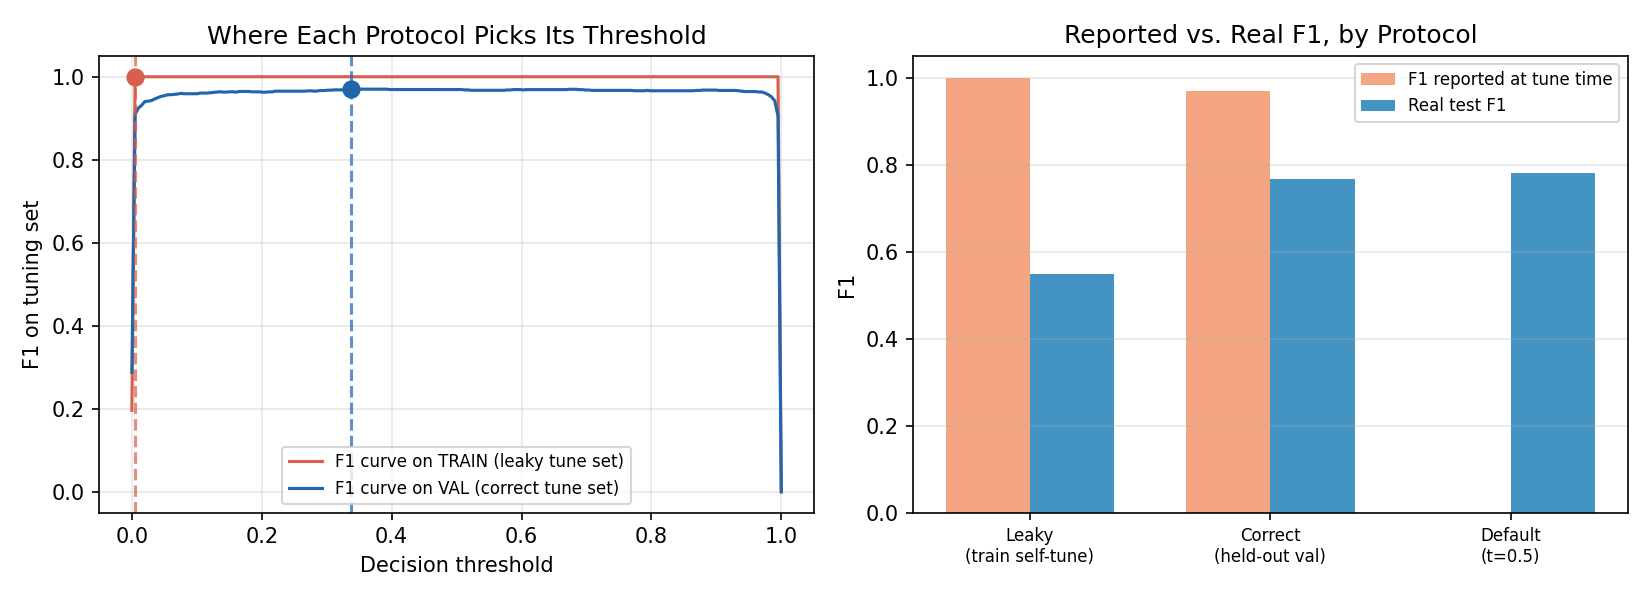
\includegraphics[width=\columnwidth]{threshold_leakage_demo.png}
  \caption{Left: F1-vs-threshold curves on the tuning set for each
           protocol; the leaky curve is tuned on training data the model
           has already fit, the correct curve on genuinely unseen
           steps~30--34. Right: F1 reported at tune time vs.\ the real
           test F1 each threshold choice actually achieves.}
  \label{fig:threshold-leakage}
\end{figure}

\textbf{The leaky protocol collapses the threshold to 0.005 and reports a
perfect F1~=~1.0 -- a model that appears flawless on paper achieves only
F1~=~0.5484 on the real test set, a 0.45 F1 illusion.} A boosted-tree
ensemble with $n{=}245$, depth~8 fits its own training set almost
perfectly (predicted probabilities cluster near 0 or 1 for training rows),
so nearly any threshold above the score floor separates the training
classes with F1 near 1 -- this is pure overfitting measured against
itself, not a discovered decision rule.

\textbf{Even the "correct" protocol is not free of drift-driven
optimism.} Tuning on the genuinely held-out val slice (steps~30--34)
avoids self-fit leakage but still reports F1~=~0.9701 at tune time against
a real test F1 of 0.7670 (0.20 gap) -- because val's illicit rate
(16.8\,\%) is closer to train's (10.9\,\%) than to test's post-drift rate
(6.5\,\%, \S\ref{sec:dataset}). Notably, the untuned default threshold
($t{=}0.5$) achieves the \emph{best} real test F1 of the three
(0.7801) -- under severe concept drift, a threshold optimized on any
pre-drift data (train or val) can transfer worse than no tuning at all.
This is the sharper, more general version of the finding: it is not
merely that self-tuning on train is wrong (obviously so), but that
\emph{any} threshold selection under temporal distribution shift should
be validated against a slice that matches the deployment regime as
closely as possible, and its transfer gap (tune-time F1 minus real
test F1) should always be reported alongside the threshold itself. Papers
that report only a tuned F1 without this gap -- common practice across the
AML literature we surveyed in \S\ref{sec:leakage} -- cannot be taken at
face value.

% ─────────────────────────────────────────────────────────────────────────────
\subsection{Inference Runtime and Scalability}
\label{sec:runtime}

For production AML screening, throughput matters as much as F1: a
transaction-monitoring pipeline scores every incoming transaction, so
per-transaction latency sets a hard ceiling on volume.
\texttt{scripts/runtime\_benchmark.py} measures batch-amortized inference
time on the same 16{,}670-row temporal test set, GPU~=~RTX~5070~Ti
(GraphSAGEv2 only; GBM is CPU/sklearn).

\begin{table}[htbp]
\centering
\caption{Inference Latency (batch-amortized, ms/transaction)}
\label{tab:runtime}
\renewcommand{\arraystretch}{1.1}
\begin{tabular}{@{}lrl@{}}
\toprule
Model & ms/tx & Notes \\
\midrule
GBM Optuna (165 feat)         & 0.0071 & \texttt{predict\_proba}, CPU \\
GBM+Structural, model only    & 0.0076 & \texttt{predict\_proba}, CPU \\
GBM+Structural, incl.\ graph feat.\ & 0.0299 & +7-feature graph pass, no cache \\
GraphSAGEv2                   & 0.0002 & full-graph forward, batched, GPU \\
\bottomrule
\end{tabular}
\end{table}

\begin{figure}[htbp]
  \centering
  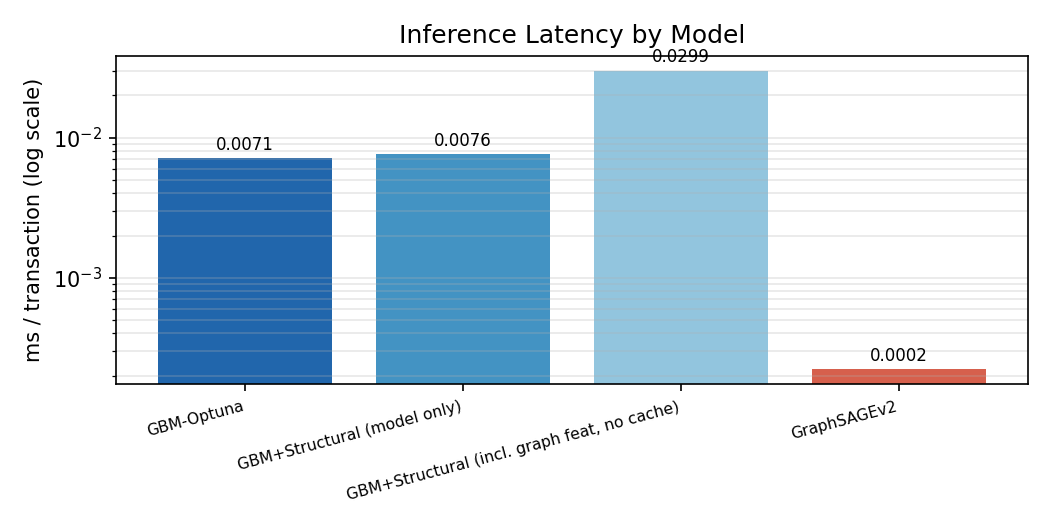
\includegraphics[width=\columnwidth]{runtime_benchmark.png}
  \caption{Inference latency by model, log scale. All four models score
           well under 1\,ms/tx in batch mode; differences span two orders
           of magnitude.}
  \label{fig:runtime}
\end{figure}

Both tree models score in single-digit microseconds per transaction --
16{,}670 rows classify in $\approx$0.12\,s total, no GPU required.
GraphSAGEv2's 0.0002\,ms/tx figure is the batched cost of one forward pass
scoring all 203{,}769 graph nodes simultaneously ($\approx$45\,ms total,
median of 20 runs); it is \emph{not} the cost of scoring one new
transaction online. In a streaming deployment, a single incoming
transaction requires materializing its $k$-hop neighborhood subgraph before
the forward pass can run -- an operation this benchmark does not isolate
and which scales with local graph density, not dataset size. The
structural-feature graph pass (degree, clustering, ego-density, OddBall)
for GBM+Structural took 4.55\,s for the full 203{,}769-node graph
(0.022\,ms/tx amortized); like GraphSAGE's neighborhood assembly, this is a
whole-graph operation that would need incremental/cached updates rather
than full recomputation per scoring pass in production. \textbf{Practical
takeaway:} the tabular GBM is the only model here with a genuinely
O(1)-per-transaction production cost; both graph-aware models carry a
graph-maintenance cost that this benchmark surfaces but does not fully
characterize for online (one-transaction-at-a-time) serving.

% ─────────────────────────────────────────────────────────────────────────────
\subsection{Explainability}
\label{sec:explain}

\begin{table}[htbp]
\centering
\caption{Cross-Model Feature Agreement (top-20 lists)}
\label{tab:shap}
\renewcommand{\arraystretch}{1.1}
\begin{tabular}{@{}lp{5.0cm}@{}}
\toprule
Agreement & Features \\
\midrule
RF $\cap$ GBM (7) &
  \texttt{lf\_18}, \texttt{lf\_47}, \texttt{lf\_53},
  \texttt{lf\_59}, \texttt{lf\_76}, \texttt{lf\_90}, \texttt{af\_70} \\[2pt]
RF $\cap$ GBM $\cap$ GNN (3) &
  \textbf{\texttt{lf\_53}}, \textbf{\texttt{lf\_90}},
  \textbf{\texttt{af\_70}} \\
\bottomrule
\end{tabular}
\end{table}

SHAP TreeExplainer was applied to GBM (Optuna, the best tabular model,
F1~=~0.824) and RF; gradient attribution was computed for GraphSAGE by
backpropagating the illicit-class logit to the input and averaging over
illicit test nodes.  Fig.~\ref{fig:shap_beeswarm} shows the GBM beeswarm
as the primary explainability view.

Three features---\texttt{lf\_53}, \texttt{lf\_90} (local), and
\texttt{af\_70} (aggregated neighborhood)---rank top-20 in every model
family.  Their cross-paradigm consensus validates them as genuine signals,
not model-specific artifacts.  The presence of the aggregated feature
\texttt{af\_70} in GNN attribution confirms that graph structure encodes
real anomaly signal.

\textbf{Answer to RQ4}: robust cross-paradigm signals exist spanning both
local transaction statistics and neighborhood aggregates.  Identifying their
semantics via Elliptic collaboration is the primary open question.

\begin{figure}[htbp]
  \centering
  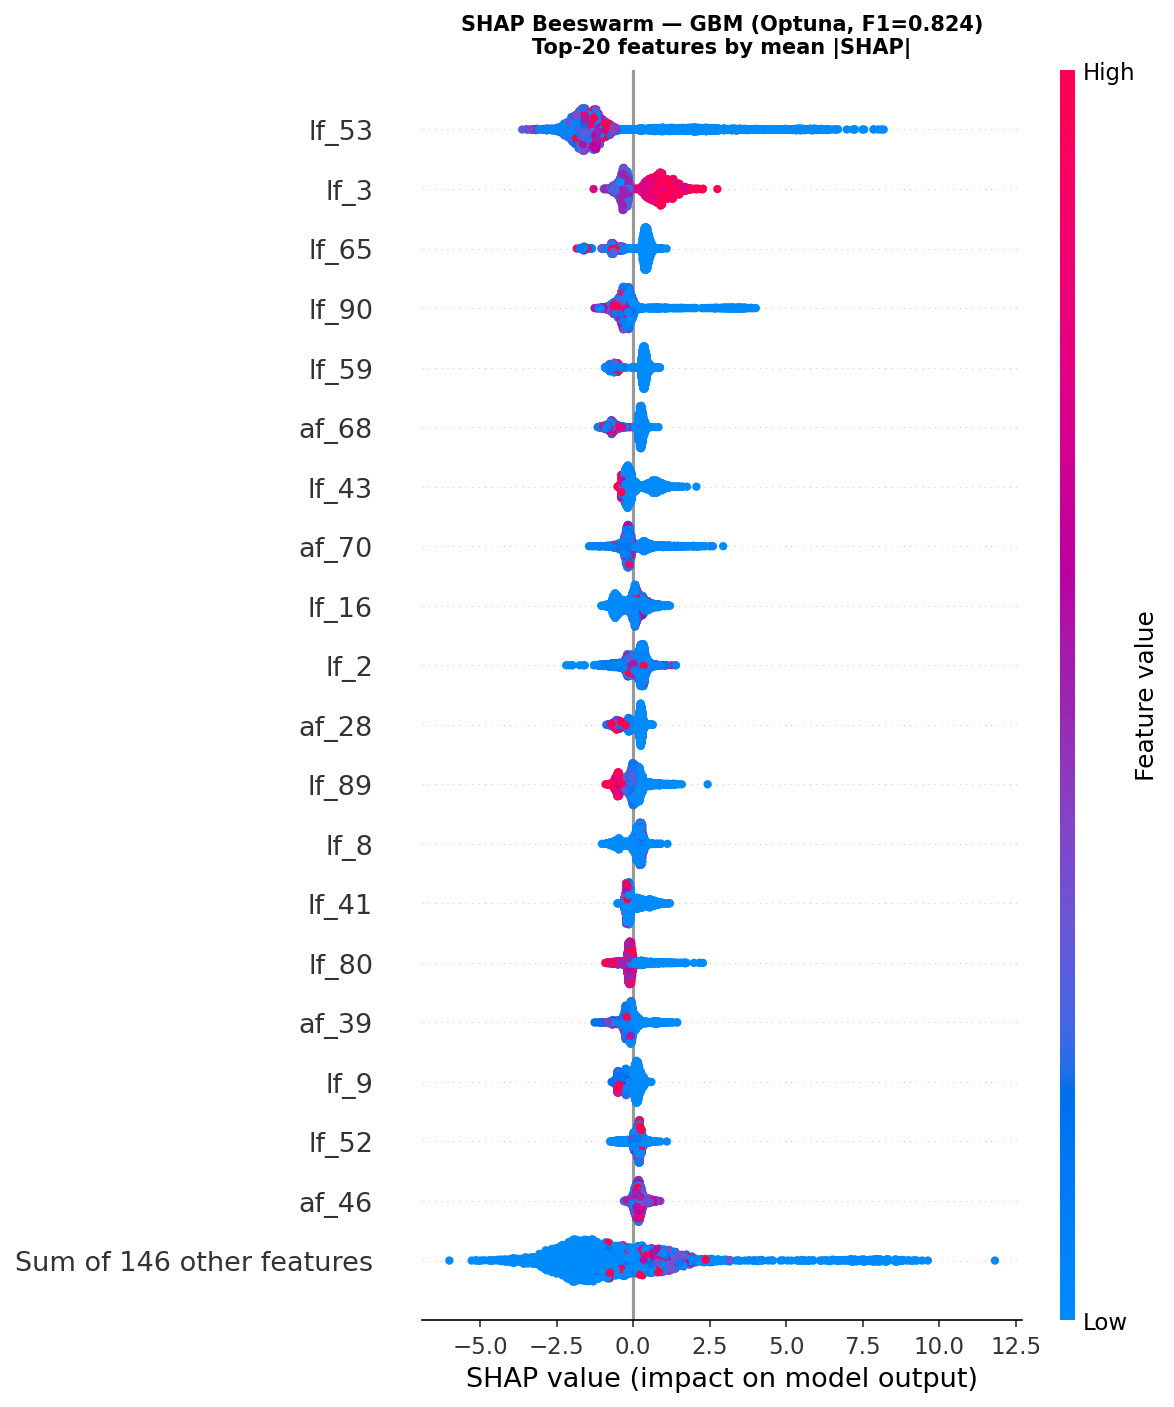
\includegraphics[width=\columnwidth]{shap_gbm_beeswarm.png}
  \caption{SHAP beeswarm for GBM (Optuna, F1~=~0.824), the best
           tabular model.  Each dot is one test-set transaction (sample
           of 3\,000); color encodes feature value (red=high, blue=low).
           Positive SHAP pushes toward illicit; negative toward licit.
           Features \texttt{lf\_53}, \texttt{lf\_90}, and \texttt{af\_70}
           rank in the top band and appear consistently across RF, GBM,
           and GraphSAGE gradient attribution.}
  \label{fig:shap_beeswarm}
\end{figure}

\begin{figure}[htbp]
  \centering
  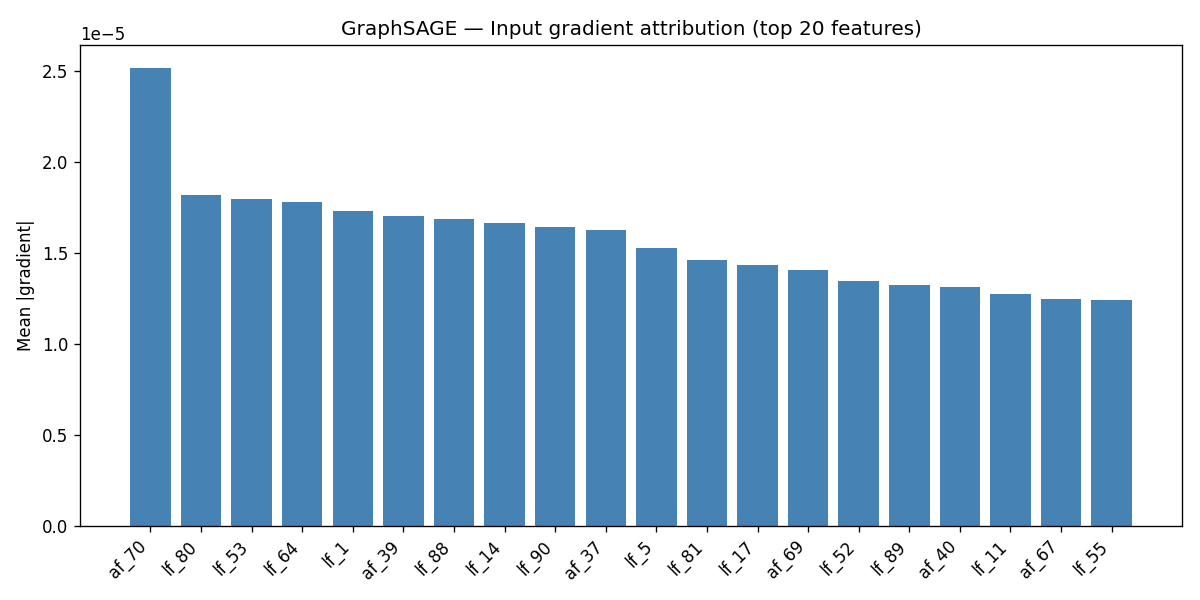
\includegraphics[width=\columnwidth]{gnn_gradient_attribution.png}
  \caption{GraphSAGE gradient attribution: mean absolute gradient per
           feature, averaged over illicit test nodes.  Features
           \texttt{lf\_53}, \texttt{lf\_90}, and \texttt{af\_70} are
           prominent despite the entirely different learning mechanism,
           confirming the cross-paradigm consensus.}
  \label{fig:gnn_attr}
\end{figure}

% ─────────────────────────────────────────────────────────────────────────────
\subsection{Error Analysis: What GBM Misses}
\label{sec:error}

We break down GBM (Optuna, tabular-only) test predictions into
TP/FP/FN/TN (\texttt{scripts/error\_analysis.py}) to characterize the
296 illicit transactions it misses (recall~=~0.727, precision~=~0.952 at
the default 0.5 threshold -- precision is high; false negatives, not false
alarms, are the dominant error mode).

\begin{figure}[htbp]
  \centering
  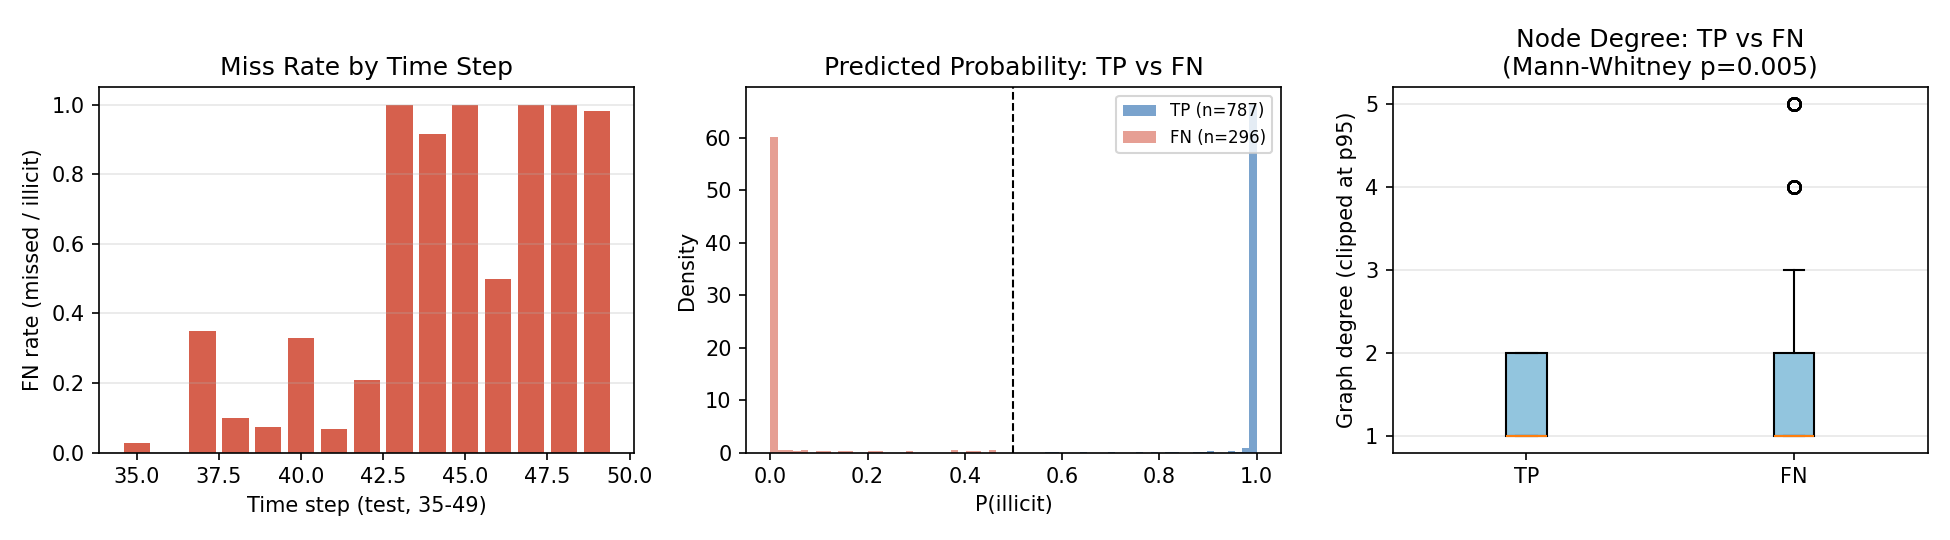
\includegraphics[width=\columnwidth]{error_analysis.png}
  \caption{Left: false-negative rate by test time step. Middle: predicted
           probability distribution, true positives vs.\ false negatives.
           Right: graph degree, true positives vs.\ false negatives.}
  \label{fig:error}
\end{figure}

\textbf{Misses concentrate almost entirely after the step-43 regime
change.} FN rate is 0--35\,\% for steps~35--42, then jumps to
92--100\,\% for steps~43--45 and~47--49 (step~46 has only 2 illicit
nodes). This step-43 boundary coincides with a real external event: prior
work on the Elliptic dataset attributes a documented dark-market shutdown
at step~43 to the sharp illicit-rate collapse (11.6\,\%$\to$6.5\,\%,
falling as low as 0.3\,\% by step~46) that defines our train/test split
(\S\ref{sec:leakage}). GBM was trained on steps~1--34, before this event;
the illicit transactions it fails to catch afterward likely reflect a
\emph{different laundering typology} than the templated pre-shutdown
patterns the model learned, not a generic recall weakness.

\textbf{Misses are confidently wrong, not borderline.} FN mean predicted
probability is 0.014 (median~0.000); 95.6\,\% of FN are scored below 0.10,
and only 2.0\,\% sit above the 0.3 "would-flag-under-a-lower-threshold"
zone. Lowering the decision threshold would recover almost none of these
296 transactions -- the model is not narrowly missing them near the
boundary, it has learned that they resemble the licit class. This rules
out threshold recalibration as a fix and points instead to concept-drift
retraining or online learning as the correct remediation.

\textbf{Graph degree is a statistically significant but practically weak
signal.} FN median degree (1.0) equals TP median degree (1.0); means
differ narrowly (1.80 vs.\ 2.01, Mann-Whitney $p{=}0.0053$). The
significance is a large-$n$ artifact, not a usable operational signal --
missed illicit transactions are not meaningfully more isolated in the
graph than caught ones, which is consistent with \S\ref{sec:leakage}'s
finding that graph topology adds only modest signal on this dataset.

\textbf{The three cross-paradigm robust features separate FN from TP.}
\texttt{lf\_53} (FN mean~$-0.485\to0.246$ relative shift toward the licit
population, $p{=}3\times10^{-125}$), \texttt{lf\_90}
($p{=}2\times10^{-140}$), and \texttt{af\_70} ($p{=}3\times10^{-24}$) all
differ significantly between FN and TP, with FN values consistently closer
to the licit population's typical range. This is the mechanistic
explanation for the misses: the post-shutdown illicit transactions do not
just evade the decision boundary by chance, they numerically resemble
licit transactions on exactly the three features SHAP and gradient
attribution identify as most discriminative overall
(\S\ref{sec:explain}), i.e.\ the new laundering typology mimics licit
behavior on the model's most-trusted signals.

% ─────────────────────────────────────────────────────────────────────────────
\section{Discussion}
\label{sec:discussion}

\textbf{RQ1 --- Density failure.}
All classical detectors score below F1~=~0.076.  Illicit transactions are
stereotyped, not rare.  This directly contradicts the assumption of classical
anomaly detection---that anomalies are low-density outliers.  On the Bitcoin
blockchain, money-laundering patterns (chain peeling, mixing) are individually
indistinguishable from legitimate high-frequency activity.

\textbf{RQ2 --- Graph vs.\ tabular.}
GraphSAGEv2 (F1~=~0.698) recovers 84.5\,\% of GBM (F1~=~0.824).  The
remaining 15.5\,\% gap reflects the richer signal encoded in the 71
pre-computed aggregated features available to tree models.  A stacking
ensemble of GBM + GraphSAGEv2 is the natural next step.

\textbf{RQ3 --- GNN design.}
LayerNorm+self-loops ($+0.068$) $>$ depth ($+0.038$) $>$ width ($+0.052$
total) $>$ learning-rate tuning ($+0.007$).  Mean aggregation dominates
attention on sparse graphs.

\textbf{RQ4 --- Robust features.}
\texttt{lf\_53}, \texttt{lf\_90}, \texttt{af\_70} are top-20 across all
model families.  The aggregated feature \texttt{af\_70} in GNN attribution
confirms that graph neighborhood signal is captured independently by tabular
proxies in tree models.

\textbf{Autoencoder paradox.}
Illicit transactions are \emph{more} regular than licit ones.  Score
inversion (low MSE = anomaly) must be validated on labeled data before
deploying any reconstruction-based AML system.

\textbf{$\beta$-VAE.}
Lower $\beta$ preserves reconstruction dominance; $\beta{\ge}2$ compresses
licit and illicit representations together.  The ceiling at F1~$\approx$~0.41
is the fundamental limit of unsupervised reconstruction-based detection here.

\textbf{Semi-supervised pseudo-labels.}
GBM gains $\Delta{=}-0.0006$: supervised boundary is already saturated.
GraphSAGEv2 gains $+0.031$: extra pseudo-labeled nodes populate graph
neighborhoods during message passing.

\textbf{Concept drift.}
Illicit rate drops from 11.6\,\% to 6.5\,\% over 15 steps.  Production
systems need temporal threshold recalibration; practical strategies include
sliding-window F1 re-optimization on the most recent labeled window,
Bayesian prior-shift correction, and adaptive class-weight schedules tied
to rolling illicit-rate estimates.

\textbf{Limitations.}
(1)~Feature semantics unknown; robust features cannot be interpreted without
Elliptic collaboration.
(2)~GAT Optuna tuning incomplete; recent Elliptic work with Chebyshev
convolutions and skip-connected GATv2 reports higher GNN F1 under
different feature subsets, so our GNN results represent a strong but not
exhaustive upper bound.
(3)~GBM + GraphSAGEv2 stacking unexplored.
(4)~DOMINANT with more epochs and $\alpha$ tuning may gain further.
(5)~Per-transaction LSTM-AE (vs.\ timestep aggregate) not evaluated.
(6)~This work positions itself as a comprehensive baseline benchmark
across paradigms; direct comparison to reported Elliptic state-of-the-art
(e.g., Chebyshev-GCN, N2V-GCN) is left for future work.

% ─────────────────────────────────────────────────────────────────────────────
\section{Conclusion}

We benchmarked 48 model variants on the Elliptic dataset across five
improvement rounds.  Six actionable findings:

\begin{enumerate}
  \item \textbf{Temporal split is mandatory.}  Random shuffling leaks future
        patterns; the 11.6\,\%$\to$6.5\,\% illicit-rate drift is real.
  \item \textbf{Supervised trees dominate.}  GBM + structural topology
        reaches F1~=~0.827; 71 aggregated features encode enough graph
        signal to outperform unsupervised GNNs.
  \item \textbf{GNNs add complementary structure.}  GraphSAGEv2 reaches
        F1~=~0.698 using only graph topology.  3-layer mean aggregation
        with LayerNorm and self-loops is optimal; GAT consistently
        underperforms on sparse graphs.
  \item \textbf{Reconstruction detection is viable but inverted.}
        $\beta$-VAE ($\beta{=}0.01$, F1~=~0.407) is the best unsupervised
        non-graph method.  Score direction must be validated before deployment.
  \item \textbf{DOMINANT is the best unsupervised graph-autoencoder method.}
        F1~=~0.212, AUC~=~0.669, exceeding all classical density detectors
        by $>$0.13 F1 ($\beta$-VAE, tabular, reaches F1~=~0.407).
  \item \textbf{Three features are cross-paradigm robust.}
        \texttt{lf\_53}, \texttt{lf\_90}, \texttt{af\_70} rank top-20 in
        RF, GBM (SHAP), and GraphSAGE (gradient attribution).
\end{enumerate}

\textbf{Future work}: (1)~GBM + GraphSAGEv2 stacking ensemble;
(2)~per-transaction LSTM-AE; (3)~EvolveGCN~\cite{pareja2020evolve} for
temporal drift; (4)~online threshold recalibration;
(5)~GNNExplainer for node-level attribution;
(6)~Elliptic collaboration to identify feature semantics.

% ─────────────────────────────────────────────────────────────────────────────
\begin{thebibliography}{99}

\bibitem{weber2019}
M.~Weber et al., ``Anti-money laundering in Bitcoin: Experimenting with graph
convolutional networks for financial forensics,'' \textit{KDD Workshop on
Anomaly Detection in Finance}, 2019.

\bibitem{pareja2020evolve}
A.~Pareja et al., ``EvolveGCN: Evolving graph convolutional networks for
dynamic graphs,'' \textit{AAAI}, 2020.

\bibitem{hamilton2017}
W.~L.~Hamilton, Z.~Ying, and J.~Leskovec, ``Inductive representation learning
on large graphs,'' \textit{NeurIPS}, 2017.

\bibitem{velickovic2018}
P.~Veli\v{c}kovi\'{c} et al., ``Graph attention networks,'' \textit{ICLR},
2018.

\bibitem{brody2022}
S.~Brody, U.~Alon, and E.~Yahav, ``How attentive are graph attention
networks?'' \textit{ICLR}, 2022.

\bibitem{ding2019dominant}
K.~Ding et al., ``Deep anomaly detection on attributed networks,''
\textit{SIAM SDM}, 2019.

\bibitem{higgins2017beta}
I.~Higgins et al., ``$\beta$-VAE: Learning basic visual concepts with a
constrained variational framework,'' \textit{ICLR}, 2017.

\bibitem{hawkins2002}
S.~Hawkins et al., ``Outlier detection using replicator neural networks,''
\textit{DaWaK}, 2002.

\bibitem{zhou2017}
C.~Zhou and R.~C.~Paffenroth, ``Anomaly detection with robust deep
autoencoders,'' \textit{KDD}, 2017.

\bibitem{vincent2008}
P.~Vincent et al., ``Extracting and composing robust features with denoising
autoencoders,'' \textit{ICML}, 2008.

\bibitem{kingma2014}
D.~P.~Kingma and M.~Welling, ``Auto-encoding variational Bayes,''
\textit{ICLR}, 2014.

\bibitem{liu2008}
F.~T.~Liu, K.~M.~Ting, and Z.-H.~Zhou, ``Isolation forest,''
\textit{IEEE ICDM}, 2008.

\bibitem{lundberg2017}
S.~M.~Lundberg and S.-I.~Lee, ``A unified approach to interpreting model
predictions,'' \textit{NeurIPS}, 2017.

\bibitem{akiba2019}
T.~Akiba et al., ``Optuna: A next-generation hyperparameter optimization
framework,'' \textit{KDD}, 2019.

\bibitem{siffer2017}
A.~Siffer, P.-A.~Fouque, A.~Termier, and C.~Largouet, ``Anomaly detection
in streams with extreme value theory,'' \textit{KDD}, 2017.

\bibitem{lee2013pseudo}
D.-H.~Lee, ``Pseudo-label: The simple and efficient semi-supervised learning
method for deep neural networks,'' \textit{ICML Workshop}, 2013.

\bibitem{alarab2020}
I.~Alarab, S.~Prakoonwit, and M.~I.~Nacer, ``Competence of graph
convolutional networks for anti-money laundering in Bitcoin blockchain,''
\textit{ICMLSC}, 2020.

\bibitem{maganti2026}
S.~Maganti, ``When graph structure becomes a liability: A critical
re-evaluation of graph neural networks for Bitcoin fraud detection under
temporal distribution shift,'' \textit{arXiv:2604.19514}, 2026.

\end{thebibliography}

\end{document}
